\begin{standout}[第一章]
    线性结构\\
    Linear Structures
\end{standout}

\begin{frame}{大纲}
    \setbeamertemplate{section in toc}[sections numbered]
    % \begin{multicols}{2}
    \tableofcontents
    % \end{multicols}
\end{frame}

\section{引例}

\begin{frame}
    \frametitle{\insertsectionhead}
    \begin{exampleblock}{引例:一元多项式的表示与计算}
        \begin{itemize}
            \item 考察一元$n$次多项式
                \[
                    f(x) = a_{0} + a_{1}x + \cdots + a_{n-1}x^{n-1} + a_{n}x^{n}
                \]
            \item 如何表示$f(x)$?
            \begin{itemize}
                \item 多项式的阶数$n$
                \item 各项系数$a_{k}$与指数$k$,其中$k\in\mathbb{Z}\cap[0,n]$
            \end{itemize}
            \item 如何对$f(x)$与$g(x)$两个多项式做基本运算?
            \begin{itemize}
                \item $f(x) \pm g(x)$
                \item $f(x) \cdot g(x)$
            \end{itemize}
        \end{itemize}
    \end{exampleblock}
\end{frame}

\begin{fragile}
    \frametitle{\insertsectionhead}
    \begin{block}{解决方案甲:利用顺序存储结构直接表示}
        \begin{itemize}
            \item 利用数组\alert{元素}与\alert{下标}分别表示多项式中对应各项的\alert{系数}与\alert{指数}
            \item 即:令数组元素\mintinline{c}{a[k]}表示$x^{k}$前的系数$a_{k}$
            \item 简单四则运算只需在数组对应元素之间运算即可
        \end{itemize}
    \end{block}
    \pause
    \begin{exampleblock}{例}
        \begin{itemize}
            \item 多项式$f(x) = 1 - 3x^{2} + 4x^{6}$与$g(x) = x + 5x^{2} -
                  7x^{4}$可分别由数组\mintinline{c}{a[]}与\mintinline{c}{b[]}表
                  示
                \pause
                \begin{figure}
                    \centering
                    \begin{bytefield}{1}
                        \bitbox[]{2}{}\bitboxes[]{3}{{\tiny$0$}{\tiny$1$}{\tiny$2$}{\tiny$3$}{\tiny$4$}{\tiny$5$}{\tiny$6$}{\tiny$\dots$}} \\
                        \bitbox[]{2}{\raggedleft\mintinline{c}{a}$\;\,$}\bitboxes{3}{{$1$}{$0$}{$-3$}{$0$}{$0$}{$0$}{$4$}{$\dots$}} \\
                        \bitbox[]{2}{\raggedleft\mintinline{c}{b}$\;\,$}\bitboxes{3}{{$0$}{$1$}{$5$}{$0$}{$-7$}{$0$}{$0$}{$\dots$}}
                    \end{bytefield}
                    \caption{解决方案甲示例演示}
                    \label{fig:demo_solution_a}
                \end{figure}
                \vspace{-2ex}
                \pause
            \item \alert{思考}:如何处理系数过于稀疏的情况?如:$f(x) = 1 - 3x^{100} + 2x^{1,000,000}$
        \end{itemize}
    \end{exampleblock}
\end{fragile}

\begin{fragile}
    \frametitle{\insertsectionhead}
    \begin{block}{解决方案乙:利用顺序存储结构只表示非零项}
        \begin{itemize}
            \item 利用数组元素表示由各\alert{非零项}的系数与指数组成的二元组$(a_{k},k)$
            \item 数组元素按非零项指数大小顺序排列
            \item 在运算时只需逐个比较每项的指数即可
        \end{itemize}
    \end{block}
    \pause
    \begin{exampleblock}{例}
        \begin{itemize}
            \item 多项式$f(x) = 9x^{12} + 15x^{8} + 3x^{2}$与$g(x) = 26x^{19} - 4x^{8} -
                  13x^{6} + 82$相加可表示为
                  \pause
                  \begin{figure}
                      \centering
                      \begin{bytefield}{1}
                          \bitbox[]{4}{}\bitboxes[]{5}{{\tiny$0$}{\tiny$1$}{\tiny$2$}{\tiny$3$}{\tiny$4$}{\tiny$5$}{\tiny$\dots$}} \\
                          \bitbox[]{4}{\raggedleft$f(x)\;\,$}\bitboxes{5}{{$(9,12)$}{$(15,8)$}{$(3,2)$}{$\dots$}} \\
                          \bitbox[]{4}{\raggedleft$g(x)\;\,$}\bitboxes{5}{{$(26,19)$}{$(-4,8)$}{$(-13,6)$}{$(82,0)$}{$\dots$}} \\
                          \bitbox[]{4}{\raggedleft$f + g\;\,$}\bitboxes{5}{{\only<4->{$(26,19)$}}{\only<5->{$(9,12)$}}{\only<6->{$(11,8)$}}{\only<7->{$(-13,6)$}}{\only<8->{$(3,2)$}}{\only<9->{$(82,0)$}}{\only<10->{$\dots$}}}
                      \end{bytefield}
                      \caption{解决方案乙示例演示过程}
                      \label{fig:demo_solution_b}
                  \end{figure}
                  \vspace{-2ex}
            \item<11> 于是,$f(x) + g(x) = 26x^{19} + 9x^{12} + 11x^{8} - 13x^{6} +
                  3x^{2} + 82$
        \end{itemize}
    \end{exampleblock}
\end{fragile}

\begin{fragile}
    \frametitle{\insertsectionhead}
    \begin{block}{解决方案丙:利用链式存储结构只表示非零项}
        \begin{figure}
            \centering
            \begin{bytefield}[boxformatting=\baselinealign]{1}
                \bitbox{10}{\mintinline{c}{coefficient}}\bitbox{8}{\mintinline{c}{exponent}}\bitbox{6}{\mintinline{c}{next}}
            \end{bytefield}
            \caption{单链表结点结构}
            \label{fig:demo_node_structure}
        \end{figure}
        \vspace{-4ex}
        \begin{itemize}
            \item 利用链表结点表示各非零项的\alert{系数}、\alert{指数}与
                  \alert{下一个}结点的地址
        \end{itemize}
    \end{block}
    \pause
    \begin{exampleblock}{例}
        \begin{itemize}
            \item 多项式$f(x) = 9x^{12} + 15x^{8} + 3x^{2}$与$g(x) = 26x^{19} - 4x^{8} -
            13x^{6} + 82$可分别表示为
        \end{itemize}
        \begin{figure}
            \centering
            \begin{bytefield}{2}
                \bitbox[]{4}{$f(x)$:}\bitbox{2}{\tikzmark{saa}}\bitbox[]{2}{\tikzmark{taa}}
                \bitboxes{3}{{$9$}{$12$}}\bitbox{2}{\tikzmark{sab}}\bitbox[]{2}{\tikzmark{tab}}
                \bitboxes{3}{{$15$}{$8$}}\bitbox{2}{\tikzmark{sac}}\bitbox[]{2}{\tikzmark{tac}}
                \bitboxes{3}{{$3$}{$2$}}\bitbox{2}{\tikzmark{sad}}\bitbox[]{2}{\tikzmark{tad}} \\
                \\
                \bitbox[]{4}{$g(x)$:}\bitbox{2}{\tikzmark{sae}}\bitbox[]{2}{\tikzmark{tae}}
                \bitboxes{3}{{$26$}{$19$}}\bitbox{2}{\tikzmark{saf}}\bitbox[]{2}{\tikzmark{taf}}
                \bitboxes{3}{{$-4$}{$8$}}\bitbox{2}{\tikzmark{sag}}\bitbox[]{2}{\tikzmark{tag}}
                \bitboxes{3}{{$-13$}{$6$}}\bitbox{2}{\tikzmark{sah}}\bitbox[]{2}{\tikzmark{tah}}
                \bitboxes{3}{{$82$}{$0$}}\bitbox{2}{\tikzmark{sai}}\bitbox[]{2}{\tikzmark{tai}}
            \end{bytefield}
            \begin{tikzpicture}[ >=stealth, thick, black!50, overlay, remember picture, %
                    list item/.style={draw=gray, rounded corners, thick} %
                ]
                \draw[->] ($({pic cs:{saa}})+(0,-0.03)$) to [out=0,in=180] ($({pic
                    cs:{taa}})+(0.26,-0.03)$);
                \fill ($({pic cs:{saa}})+(0,-0.03)$) circle [radius=0.05];
                \draw[->] ($({pic cs:{sab}})+(0,-0.03)$) to [out=0,in=180] ($({pic
                    cs:{tab}})+(0.26,-0.03)$);
                \fill ($({pic cs:{sab}})+(0,-0.03)$) circle [radius=0.05];
                \draw[->] ($({pic cs:{sac}})+(0,-0.03)$) to [out=0,in=180] ($({pic
                    cs:{tac}})+(0.26,-0.03)$);
                \fill ($({pic cs:{sac}})+(0,-0.03)$) circle [radius=0.05];
                % \draw[->] ($({pic cs:{sad}})+(0,-0.03)$) to [out=0,in=180] ($({pic
                %     cs:{tad}})+(0.26,-0.03)$);
                % \fill ($({pic cs:{sad}})+(0,-0.03)$) circle [radius=0.05];
                \draw[->] ($({pic cs:{sae}})+(0,-0.03)$) to [out=0,in=180] ($({pic
                    cs:{tae}})+(0.26,-0.03)$);
                \fill ($({pic cs:{sae}})+(0,-0.03)$) circle [radius=0.05];
                \draw[->] ($({pic cs:{saf}})+(0,-0.03)$) to [out=0,in=180] ($({pic
                    cs:{taf}})+(0.26,-0.03)$);
                \fill ($({pic cs:{saf}})+(0,-0.03)$) circle [radius=0.05];
                \draw[->] ($({pic cs:{sag}})+(0,-0.03)$) to [out=0,in=180] ($({pic
                    cs:{tag}})+(0.26,-0.03)$);
                \fill ($({pic cs:{sag}})+(0,-0.03)$) circle [radius=0.05];
                \draw[->] ($({pic cs:{sah}})+(0,-0.03)$) to [out=0,in=180] ($({pic
                    cs:{tah}})+(0.26,-0.03)$);
                \fill ($({pic cs:{sah}})+(0,-0.03)$) circle [radius=0.05];
                \draw ($({pic cs:{sad}})+(-0.22,-0.3)$) -- ($({pic cs:{sad}})+(0.23,0.23)$);
                \draw ($({pic cs:{sai}})+(-0.22,-0.3)$) -- ($({pic cs:{sai}})+(0.23,0.23)$);
            \end{tikzpicture}
            \caption{解决方案丙示例结构}
            \label{fig:demo_solution_c}
        \end{figure}
    \end{exampleblock}
\end{fragile}

\begin{frame}
    \frametitle{\insertsectionhead}
    \begin{alertblock}{一点启示}
        \begin{itemize}
            \item 同一问题有不同的表示方案
            \item 共性:\alert{线性结构}的组织与管理
        \end{itemize}
    \end{alertblock}
\end{frame}
\section{线性结构}

\begin{frame}
    \frametitle{\insertsectionhead}
    \begin{block}{线性结构(Linear Structure)}
        \begin{itemize}
            \item 又名\textbf{线性表}、\textbf{序列(sequence)},指具有\alert{相
                  同}数据类型的$n$个\footnote{$n\in\mathbb{Z}\cap[0,+\infty)$}数
                  据元素的\alert{有限}序列
            \item 其\textbf{长度(length)}指序列中数据元素的个数
            \item 非空序列指至少含有一个元素的序列,可记作
                \[
                    s = (a_{1}, a_{2}, \cdots, a_{k}, \cdots, a_{n}),
                \]
                其中
                \begin{itemize}
                    \item $a_{k}$表示数据元素\footnote{可表示\alert{任意}数据类
                          型,如无特别说明则采用简单数据类型}
                    \item 下标$k \in \mathbb{Z} \cap [1, n]$表示该元素在序列中的
                          位置\textbf{序号(index)}或\textbf{秩(rank)}
                \end{itemize}
            \item 特别地,空序列可记作
                \[
                    s = ()
                \]
        \end{itemize}
    \end{block}
\end{frame}

\begin{fragile}
    \frametitle{\insertsectionhead}
    \begin{exampleblock}{例:幼儿园小朋友排队放学}
        \begin{itemize}
            \item 每个班均只有\alert{有限}多个小朋友
            \item 在每个班队伍中一般不允许有不属于该班小朋友的存在
            \item 为点名方便,所有小朋友均须\alert{按顺序}排队
            \begin{itemize}
                \item 排头小朋友前面与排尾小朋友后面均没有其他小朋友
                \item 其余每个小朋友的前后均有且只有一个其他小朋友
            \end{itemize}
        \end{itemize}
    \end{exampleblock}
    \begin{figure}[h]
        \centering
        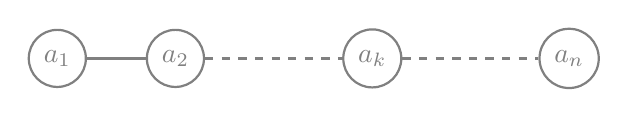
\begin{tikzpicture}[ >=stealth, thick, black!50, %
            list item/.style={draw=gray, circle, thick} %
        ]
            \node [list item] (item1) at (-3.5,0) {$a_{1}$}; %
            \node [list item] (item2) at (-2,0) {$a_{2}$}; %
            \node [list item] (itemk) at (0.5,0) {$a_{k}$}; %
            \node [list item] (itemn) at (3,0) {$a_{n}$}; %
            \draw  (item1) -- (item2); %
            \draw[dashed] (item2) -- (itemk); %
            \draw[dashed] (itemk) -- (itemn); %
        \end{tikzpicture}
        % \caption{}
        \label{fig:demo_linear_structure_kids}
    \end{figure}
\end{fragile}

\begin{frame}
    \frametitle{\insertsectionhead}
    \begin{block}{序列的特点}
        \begin{itemize}
            \item \textbf{有穷性}:序列中数据元素的个数是\alert{有限}的
            \item \textbf{一致性}:序列中所有数据元素\alert{类型}均须\alert{相
                  同}
            \item \textbf{顺序性}:序列中所有元素均按\alert{顺序}排列
            \begin{itemize}
                \item 首元素无\textbf{前驱(predecessor)},尾元素无\textbf{后继
                      (successor)}
                \item 其余元素均分别有且只有一个\textbf{直接(immediate)前驱}与
                      \textbf{直接后继}
            \end{itemize}
        \end{itemize}
    \end{block}
    \begin{figure}[h]
        \centering
        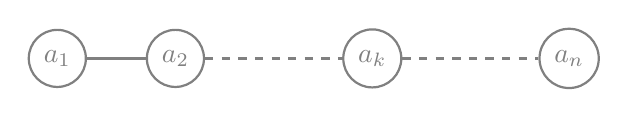
\begin{tikzpicture}[ >=stealth, thick, black!50, %
            list item/.style={draw=gray, circle, thick} %
        ]
            \node [list item] (item1) at (-3.5,0) {$a_{1}$}; %
            \node [list item] (item2) at (-2,0) {$a_{2}$}; %
            \node [list item] (itemk) at (0.5,0) {$a_{k}$}; %
            \node [list item] (itemn) at (3,0) {$a_{n}$}; %
            \draw  (item1) -- (item2); %
            \draw[dashed] (item2) -- (itemk); %
            \draw[dashed] (itemk) -- (itemn); %
        \end{tikzpicture}
        % \caption{}
        \label{fig:demo_linear_structure_kids_2}
    \end{figure}
\end{frame}

\begin{fragile}
    \frametitle{\insertsectionhead}
    \begin{block}{序列的抽象数据类型}
        \begin{minted}[linenos=false,escapeinside=@@]{c}
            ADT Sequence {
            数据:
                数据对象: @$\mathcal{D} = \{a_{k} | a_{k}\in\text{数据元素集合}, k\in\mathbb{Z}\cap[1,n]\}$@
                逻辑关系: @$\mathcal{R} = \{\langle{}a_{k-1},a_{k}\rangle | k\in\mathbb{Z}\cap[2,n]\}$@
            操作:
                create_sequence()
                    构造并初始化一个空序列@$s$@
                get_sequence_length(s)
                    获取并返回序列@$s$@中所含元素个数
                get_sequence_element(s, k)
                    获取并返回序列@$s$@中的第@$k$@个元素
                search_sequence_element(s, x)
                    查找序列@$s$@中值为@$x$@的元素, 返回其首次出现的序号或地址
                insert_sequence_element(s, k, x)
                    在序列@$s$@的第@$k$@个位置插入值为@$x$@的新元素, 后续元素序号与总元素个数均加1
                remove_sequence_element(s, k)
                    删除序列@$s$@的第@$k$@个元素, 后续元素序号与总元素个数均减1
            }
        \end{minted}
    \end{block}
\end{fragile}

\begin{frame}
    \frametitle{\insertsectionhead}
    \begin{alertblock}{一些说明}
        \begin{itemize}
            \item 线性结构的基本操作由实际应用而定
            \item 复杂操作可通过基本操作的组合而实现
            \item 针对不同应用,其操作接口可能略有差异
        \end{itemize}
    \end{alertblock}
\end{frame}

\begin{frame}
    \frametitle{\insertsectionhead}
    \begin{block}{序列的存储结构}
        \begin{itemize}
            \item 顺序存储结构:\textbf{顺序列表}
            \begin{itemize}
                \item 元素按地址相邻存储在内存的一片\alert{连续}地址空间中
                \item 长度\alert{固定},可由\textbf{内置数组}的简单封装实现
                \item 若欲实现变长结构,须采用进一步策略封装成\textbf{动态数组}
                      或\textbf{向量}
            \end{itemize}
            \item 链式存储结构:\textbf{链式列表}
            \begin{itemize}
                \item 元素在内存中一般彼此\alert{不相邻},仅按前驱后继关系通过
                      \textbf{指针}相连
                \item 长度\alert{可变},可由自定义\textbf{结构体}实现,较灵活
            \end{itemize}
        \end{itemize}
    \end{block}
\end{frame}

\subsection{顺序存储与运算实现}

\begin{fragile}
    \frametitle{\insertsubsectionhead}
    \begin{block}{顺序列表(Sequence List)}
        \begin{itemize}
            \item 又名\textbf{顺序表},用一段地址\alert{连续}的存储单
                  元,\alert{依次}存储序列中的数据元素
        \end{itemize}
    \end{block}
    \pause
    \begin{exampleblock}{例}
        \begin{itemize}
            \item 考察序列$s = (34, 23, 67, 43)$采用顺序表形式存储的过程
                  \vspace{2ex}
                \begin{figure}
                    \centering
                    \begin{bytefield}{2}
                        \bitbox[]{2}{}
                        \bitboxes[]{3}{{\only<3|handout:0>{\mintinline[fontsize=\smaller]{c}{last}}}
                            {\only<4|handout:0>{\mintinline[fontsize=\smaller]{c}{last}}}
                            {\only<5|handout:0>{\mintinline[fontsize=\smaller]{c}{last}}}
                            {\only<6>{\mintinline[fontsize=\smaller]{c}{last}}}} \\
                        \bitbox[]{2}{}
                        \bitboxes[]{3}{{\only<3>{\tikzmark{sba}}}{\only<4>{\tikzmark{sba}}}
                            {\only<5>{\tikzmark{sba}}}{\only<6>{\tikzmark{sba}}}} \\
                        \bitbox[]{2}{$s$:}
                        \bitbox{3}{\only<3->{$34$}}\bitbox{3}{\only<4->{$23$}}\bitbox{3}{\only<5->{$67$}}\bitbox{3}{\only<6->{$43$}}
                        \bitboxes{3}{{}{}{}{}}
                    \end{bytefield}
                    \begin{tikzpicture}[ >=stealth, thick, black!50, overlay, remember picture, %
                            list item/.style={draw=gray, rounded corners, thick} %
                        ]
                        \only<3->{
                            \draw[->] ($({pic cs:{sba}})+(0,0.3)$) to [out=-90,in=90] ($({pic
                                cs:{sba}})+(0,-0.3)$);
                            % \fill ($({pic cs:{saa}})+(0,-0.03)$) circle [radius=0.05];
                        }
                    \end{tikzpicture}
                    \caption{顺序表存储过程演示}
                    \label{fig:demo_sequence_list_construction}
                \end{figure}
        \end{itemize}
    \end{exampleblock}
\end{fragile}

\begin{fragile}
    \frametitle{\insertsubsectionhead}
    \begin{alertblock}{思考:用何种属性描述顺序表?}
        \begin{itemize}
            \item<2-> 存储空间的起始位置
            \item<3-> \textbf{容量(capacity)}:最多可容纳的元素个数
            \item<4-> \textbf{长度(length)}:实际容纳的元素个数
        \end{itemize}
    \end{alertblock}
    \begin{figure}
        \centering
        \begin{bytefield}[bitwidth=1em]{2}
            \bitboxes[]{6}{{\only<2->{\mintinline[fontsize=\smaller]{c}{first}}}}
            \bitboxes[]{3}{{}{}{}{}{}{}{}{}} \\
            \bitboxes[]{6}{{\only<2->{\tikzmark{sca}}}}
            \bitboxes[]{3}{{}{}{}{}{}{}{}{}} \\
            \bitbox[]{3}{$s$:}
            \bitbox{3}{$34$}\bitbox{3}{$23$}\bitbox{3}{$67$}\bitbox{3}{$43$}
            \bitboxes{3}{{}{}{}{}}
            \bitbox{2}{$4$} \\
            \bitbox[]{3}{}
            \bitbox[t]{24}{\only<3->{$\underbrace{\hspace{30em}}_{\text{容量}}$}}
            \bitbox[t]{2}{\only<4->{$\underbrace{\hspace{2em}}_{\text{长度}}$}}
        \end{bytefield}
        \begin{tikzpicture}[ >=stealth, thick, black!50, overlay, remember picture, %
                list item/.style={draw=gray, rounded corners, thick} %
            ]
            \only<2->{
                \draw[->] ($({pic cs:{sca}})+(0,0.3)$) to [out=-90,in=90] ($({pic
                    cs:{sca}})+(0,-0.3)$);
            }
        \end{tikzpicture}
        \caption{顺序表的属性描述}
        \label{fig:demo_sequence_list_properties}
    \end{figure}
\end{fragile}

\begin{fragile}
    \frametitle{\insertsubsectionhead}
    \begin{alertblock}{思考:如何为顺序表分配内存?}
        \begin{itemize}
            \item<2-> 一维数组的静态分配
        \end{itemize}
    \end{alertblock}
    \begin{figure}
        \centering
        \begin{bytefield}[bitwidth=1em]{2}
            \bitbox[]{3}{$s$:}
            \bitbox{3}{$34$}\bitbox{3}{$23$}\bitbox{3}{$67$}\bitbox{3}{$43$}
            \bitboxes{3}{{}{}{}{}}
            \bitbox{2}{$4$}
        \end{bytefield}
        \caption{顺序表的内存分配}
        \label{fig:demo_sequence_list_memory_allocation}
    \end{figure}
\end{fragile}

\begin{fragile}
    \frametitle{\insertsubsectionhead}
    \begin{alertblock}{思考:如何获取任意元素的存储地址?}
        \begin{itemize}
            \item<5-> 令$p_{k}$为元素$a_{k}$的起始地址,且每个元素$a_{k}$所占空
                  间为$m$,则有
                  \[
                        p_{k} = p_{1} + (k - 1)m, \qquad k\in\mathbb{Z}\cap[1, n]
                  \]
            \item<6> 顺序列表中的元素可被\textbf{随机访问(Random Access)},时间
                  复杂度为$O(1)$
        \end{itemize}
    \end{alertblock}
    \begin{figure}
        \centering
        \begin{bytefield}[bitwidth=1em]{2}
            \bitboxes[]{6}{{\only<2->{$p_{1}$}}{}{\only<3->{$p_{k}$}}}\bitboxes[]{17}{} \\
            \bitboxes[]{6}{{\only<2->{\tikzmark{sda}}}{}{\only<3->{\tikzmark{sdb}}}}\bitboxes[]{17}{} \\
            \bitbox[]{3}{\baselinealign{$s:$}}
            \bitbox{3}{\baselinealign{$a_{1}$}}\bitbox{6}{\baselinealign{$\cdots$}}\bitbox{3}{\baselinealign{$a_{k-1}$}}
            \bitbox{3}{\baselinealign{$a_{k}$}}\bitbox{6}{\baselinealign{$\cdots$}}\bitbox{3}{\baselinealign{$a_{n}$}}
            \bitbox{6}{\baselinealign{$\cdots$}}\bitbox{2}{\baselinealign{$n$}} \\
            \bitbox[]{3}{}
            \bitbox[t]{12}{\only<4->{$\underbrace{\hspace{15em}}_{k-1}$}}\bitbox[t]{9}{}
            \bitbox[t]{3}{\only<5->{$\underbrace{\hspace{3.5em}}_{m}$}}
        \end{bytefield}
        \begin{tikzpicture}[ >=stealth, thick, black!50, overlay, remember picture, %
                list item/.style={draw=gray, rounded corners, thick} %
            ]
            \only<2->{
                \draw[->] ($({pic cs:{sda}})+(0,0.3)$) to [out=-90,in=90] ($({pic
                    cs:{sda}})+(0,-0.3)$);
            }
            \only<3->{
                \draw[->] ($({pic cs:{sdb}})+(0,0.3)$) to [out=-90,in=90] ($({pic
                    cs:{sdb}})+(0,-0.3)$);
            }
        \end{tikzpicture}
        \caption{顺序表的随机访问原理}
        \label{fig:demo_sequence_list_random_access}
    \end{figure}
\end{fragile}

\begin{fragile}
    \frametitle{\insertsubsectionhead}
    \bicolumns[0.5]{
        \begin{block}{顺序表的类型说明}
            \begin{itemize}
                \item 以整型常量表示\alert{容量}
                \item 以静态数组存储表中各元素
                \item 以尾元素的序号加$1$表示\alert{长度}
                \item 特别地,空表尾元素序号为$-1$
            \end{itemize}
        \end{block}
    }{
        \begin{minted}{c}
            #define CAPACITY 256
            
            typedef int DataType; // 元素类型

            typedef struct {
                DataType data[CAPACITY]; // 元素
                int last; // 尾元素序号
            } SequenceList;
        \end{minted}
    }
\end{fragile}

\begin{fragile}
    \frametitle{\insertsubsectionhead}
    \bicolumns[0.45]{
        \begin{block}{顺序表的初始化}
            \begin{itemize}
                \item 为空表动态分配空间
                \item 将尾元素序号置为$-1$
                \item 返回指向空表的指针
            \end{itemize}
        \end{block}
    }{
        \begin{minted}{c}
            SequenceList *create_sequence_list() {
                SequenceList *s = malloc(sizeof(SequenceList));
                if (s) {
                    s->last = -1;
                }
                return s;
            }
        \end{minted}
    }
\end{fragile}

\begin{fragile}
    \frametitle{\insertsubsectionhead}
    \bicolumns[0.45]{
        \begin{block}{向顺序表中插入元素}
            \begin{itemize}
                \item 检测并处理非法输入\footnotemark
                \item 依次\alert{向后}移动目标位置后元素
                \item 在目标位置处插入新元素
                \item 更新尾元素序号
            \end{itemize}
        \end{block}
    }{
        \begin{minted}[highlightlines={3, 4, 8}]{c}
            bool insert_sequence_list(
                    SequenceList *s, int k, DataType d) {
                if (full_sequence_list(s)
                        || wrong_insert_index(s, k)) {
                    return false; // 检测并处理各种非法插入情况
                }
                for (int i = s->last; i >= k; --i) {
                    s->data[i + 1] = s->data[i]; // 注意移动顺序
                }
                s->data[k] = d; // 插入新元素
                ++s->last; // 更新尾元素序号
                return true;
            }
        \end{minted}
    }

    \footnotetext{为表示布尔型变量,须包含
            \mintinline[fontsize=\smaller]{c}{<stdbool.h>}头,下同}
\end{fragile}

\begin{fragile}
    \frametitle{\insertsubsectionhead}
    \begin{exampleblock}{例}
        \begin{itemize}
            \item 在顺序表形式的序列$s=(35, 12, 24, 42)$中第$1$个位置处插入$33$
        \end{itemize}
    \end{exampleblock}
    \begin{figure}
        \centering
        \begin{bytefield}[bitwidth=1em]{2}
            \bitbox[]{3}{}
            \bitboxes[]{3}{{\tiny$0$}{\tiny$1$}{\tiny$2$}{\tiny$3$}{\tiny$4$}{\tiny$5$}{\tiny$6$}{\tiny$\dots$}} \\
            \bitbox[]{3}{\baselinealign{$s:$}}
            \bitboxes{3}{
                {$35$}
                {\only<1-4|handout:0>{$12$}\only<5->{$33$}}
                {\only<1-3|handout:0>{$24$}\only<4->{$12$}}
                {\only<1-2|handout:0>{$42$}\only<3->{$24$}}
                {\only<2->{$42$}}{}{}{}} \\
            \bitboxes[]{3}{{}{}{\tikzmark{sea}}{}{\only<1-5>{\tikzmark{seb}}}{\only<6->{\tikzmark{seb}}}{}{}{}} \\
            \bitboxes[]{3}{{}{}{\only<1-4>{$33$}}{}{\only<1-5|handout:0>{\mintinline[fontsize=\smaller]{c}{last}}}{\only<6->{\mintinline[fontsize=\smaller]{c}{last}}}{}{}{}}
        \end{bytefield}
        \begin{tikzpicture}[ >=stealth, thick, black!50, overlay, remember picture, %
                list item/.style={draw=gray, rounded corners, thick} %
            ]
            \draw[->] ($({pic cs:{sea}})+(0,-0.35)$) to [out=90,in=-90] ($({pic
                cs:{sea}})+(0,0.25)$);
            \draw[->] ($({pic cs:{seb}})+(0,-0.35)$) to [out=90,in=-90] ($({pic
                cs:{seb}})+(0,0.25)$);
        \end{tikzpicture}
        \caption{在顺序表中插入元素过程演示}
        \label{fig:demo_insert_sequence_list}
    \end{figure}
\end{fragile}

\begin{frame}
    \frametitle{\insertsubsectionhead}
    \begin{block}{顺序表插入算法的复杂度分析}
        \begin{itemize}
            \item<2-> 插入运算主要耗时于\alert{依次移动数据}
                \begin{itemize}
                    \item 在序号为$k$的位置插入时须移动$n-k$
                          次,$k\in\mathbb{Z}\cap[0, n]$
                \end{itemize}
            \item<3-> 若在序号为$k$的位置插入的概率为$p_{k}$,则移动次数的期望为
                \[
                    \mathbb{E}_{\text{insert}} = \sum_{k=0}^{n}{(n - k)p_{k}}
                \]
            \item<4-> 当在所有合法位置插入的概率均等时,即对所有合法的$k$均有
                $p_{k}=(n + 1)^{-1}$,则有
                \[
                    \mathbb{E}_{\text{insert}} = \frac{1}{n + 1}\sum_{k=0}^{n}{(n - k)} = \frac{n}{2}
                \]
            \item<5-> 综上,顺序表插入操作的时间复杂度为$O(n)$
        \end{itemize}
    \end{block}
\end{frame}

\begin{fragile}
    \frametitle{\insertsubsectionhead}
    \bicolumns[0.45]{
        \begin{block}{从顺序表中删除元素}
            \begin{itemize}
                \item 检测并处理非法输入
                \item 依次\alert{向前}移动目标位置后元素
                \item \alert{覆盖}目标位置处的元素
                \item 更新尾元素序号
            \end{itemize}
        \end{block}
    }{
        \begin{minted}[highlightlines={3, 7, 10}]{c}
            bool remove_sequence_list(
                    SequenceList *s, int k, DataType *d) {
                if (wrong_remove_index(s, k)) {
                    return false; // 检测并处理各种非法插入情况
                }
                if (d) {
                    *d = s->data[k]; // 记录并返回被删的值
                }
                for (int i = k; i < s->last; ++i) {
                    s->data[i] = s->data[i + 1]; // 注意移动顺序
                }
                --s->last; // 更新尾元素序号
                return true;
            }
        \end{minted}
    }
\end{fragile}

\begin{fragile}
    \frametitle{\insertsubsectionhead}
    \begin{exampleblock}{例}
        \begin{itemize}
            \item 删除顺序表形式的序列$s=(35, 33, 12, 24, 42)$中第$1$个位置元素
                  $33$
        \end{itemize}
    \end{exampleblock}
    \begin{figure}
        \centering
        \begin{bytefield}[bitwidth=1em]{2}
            \bitbox[]{3}{}
            \bitboxes[]{3}{{\tiny$0$}{\tiny$1$}{\tiny$2$}{\tiny$3$}{\tiny$4$}{\tiny$5$}{\tiny$6$}{\tiny$\dots$}} \\
            \bitbox[]{3}{\baselinealign{$s:$}}
            \bitboxes{3}{
                {$35$}
                {\only<2->{$12$}\only<1|handout:0>{$33$}}
                {\only<3->{$24$}\only<1-2|handout:0>{$12$}}
                {\only<4->{$42$}\only<1-3|handout:0>{$24$}}
                {\only<1->{$42$}}{}{}{}} \\
            \bitboxes[]{3}{{}{}{\tikzmark{sfa}}{}{\only<5->{\tikzmark{sfb}}}{\only<1-4|handout:0>{\tikzmark{sfb}}}{}{}{}} \\
            \bitboxes[]{3}{{}{}{\only<2->{$33$}}{}{\only<5->{\mintinline[fontsize=\smaller]{c}{last}}}{\only<1-4|handout:0>{\mintinline[fontsize=\smaller]{c}{last}}}{}{}{}}
        \end{bytefield}
        \begin{tikzpicture}[ >=stealth, thick, black!50, overlay, remember picture, %
                list item/.style={draw=gray, rounded corners, thick} %
            ]
            \draw[->] ($({pic cs:{sfa}})+(0,-0.35)$) to [out=90,in=-90] ($({pic
                cs:{sfa}})+(0,0.25)$);
            \draw[->] ($({pic cs:{sfb}})+(0,-0.35)$) to [out=90,in=-90] ($({pic
                cs:{sfb}})+(0,0.25)$);
        \end{tikzpicture}
        \caption{从顺序表中删除元素过程演示}
        \label{fig:demo_remove_sequence_list}
    \end{figure}
\end{fragile}

\begin{frame}
    \frametitle{\insertsubsectionhead}
    \begin{block}{顺序表删除算法的复杂度分析}
        \begin{itemize}
            \item<2-> 删除与插入运算互为逆运算,故仍主要耗时于\alert{依次移动数据}
            \item<3-> 同理可得顺序表删除操作的时间复杂度亦为$O(n)$
        \end{itemize}
    \end{block}
\end{frame}

\begin{fragile}
    \frametitle{\insertsubsectionhead}
    \bicolumns[0.45]{
        \begin{block}{在顺序表中按值查找元素}
            \begin{itemize}
                \item 从首至尾遍历表中所有元素
                \item 若发现匹配元素则返回其序号
                \item 否则返回$-1$表示查找失败
            \end{itemize}
        \end{block}
    }{
        \begin{minted}{c}
            int search_sequence_list(SequenceList *s, DataType d) {
                int k = 0;
                for (; k <= s->last && s->data[k] != d; ++k)
                    ; // 空语句,不执行任何操作
                return s->last < k ? -1 : k;
            }
        \end{minted}
    }
\end{fragile}

\begin{fragile}
    \frametitle{\insertsubsectionhead}
    \begin{exampleblock}{例}
        \begin{itemize}
            \item 在顺序表形式的序列$s=(35, 33, 12, 24, 42)$查找值为$12$的元素的
                  位置
        \end{itemize}
    \end{exampleblock}
    \begin{figure}
        \centering
        \begin{bytefield}[bitwidth=1em]{2}
            \bitbox[]{3}{}
            \bitboxes[]{3}{{\tiny$0$}{\tiny$1$}{\tiny$2$}{\tiny$3$}{\tiny$4$}{\tiny$5$}{\tiny$6$}{\tiny$\dots$}} \\
            \bitbox[]{3}{\baselinealign{$s:$}}
            \bitboxes{3}{{$35$}{$33$}{\alert<5>{$12$}}{$24$}{$42$}{}{}{}} \\
            \bitboxes[]{3}{{}{\only<2>{\tikzmark{sga}}}{\only<3>{\tikzmark{sga}}}{\only<4->{\tikzmark{sga}}}{}{}{}}
        \end{bytefield}
        \begin{tikzpicture}[ >=stealth, thick, black!50, overlay, remember picture, %
                list item/.style={draw=gray, rounded corners, thick} %
            ]
            \only<2->{
                \draw[->] ($({pic cs:{sga}})+(0,-0.35)$) to [out=90,in=-90] ($({pic
                    cs:{sga}})+(0,0.25)$);
            }
        \end{tikzpicture}
        \caption{在顺序表中查找元素过程演示}
        \label{fig:demo_search_sequence_list}
    \end{figure}
\end{fragile}

\begin{frame}
    \frametitle{\insertsubsectionhead}
    \begin{alertblock}{课堂思考练习}
        \begin{itemize}
            \item<2-> 分析顺序表删除算法的时间复杂度
            \item<3-> 实现逆序遍历搜索并讨论其与顺序遍历的异同
        \end{itemize}
    \end{alertblock}
\end{frame}

\begin{frame}
    \frametitle{\insertsubsectionhead}
    \begin{block}{顺序表的优势}
        \begin{itemize}
            \item 节省空间:无需为表示元素间逻辑关系而增加额外存储空间
            \item 随机访问:可快速访问表中任意位置元素,$T(n) = O(1)$
        \end{itemize}
    \end{block}
    \pause
    \begin{block}{顺序表的不足}
        \begin{itemize}
            \item 容量固定:表容量事先难以确定且难以扩充
            \item 增减困难:插入删除元素需移动大量元素,$T(n) = O(n)$
        \end{itemize}
    \end{block}
\end{frame}

\begin{frame}
    \frametitle{\insertsubsectionhead}
    \begin{alertblock}{课堂编程练习}
        \begin{itemize}
            \item 输入:顺序表$s_{a}$与$s_{b}$,其元素均已按\alert{升序}排列
            \item 输出:顺序表$s_{c}$,其元素为$s_{a}$与$s_{b}$中元素的合并,并
                  以\alert{降序}排列
        \end{itemize}
    \end{alertblock}
\end{frame}
\subsection{链式存储与运算实现}

\begin{frame}
    \frametitle{\insertsubsectionhead}
    \begin{block}{链式列表(Linked List)}
        \begin{itemize}
            \item 简称\textbf{链表},用一组在内存中\alert{零散}分布的存储单元存
                  储序列中的数据元素
            \item 按链接关系分为\textbf{单向链表}\footnote{简称\textbf{单链
                  表}}、\textbf{双向链表}与\textbf{循环链表}等
        \end{itemize}
    \end{block}
    \pause
    \begin{exampleblock}{例}
        \begin{itemize}
            \item 考察序列$s = (34, 23, 67, 43)$采用\alert{单链表}形式存储的过程
        \end{itemize}
        \begin{figure}
            \centering
            \begin{bytefield}{2}
                \bitbox[]{3}{}
                \bitbox[]{3}{\mintinline[fontsize=\smaller]{c}{head}}
                \bitbox[]{30}{} \\
                \bitbox[]{3}{}
                \bitbox[]{3}{\only<2->{\tikzmark{shf}}}
                \bitbox[]{30}{} \\
                \bitbox[]{3}{$s:$}
                \bitbox{3}{}\bitbox{2}{\tikzmark{sha}}\bitbox[]{2}{\tikzmark{tha}}
                \uncover<3->{\bitbox{3}{$34$}\bitbox{2}{\tikzmark{shb}}\bitbox[]{2}{\tikzmark{thb}}}
                \uncover<4->{\bitbox{3}{$23$}\bitbox{2}{\tikzmark{shc}}\bitbox[]{2}{\tikzmark{thc}}}
                \uncover<5->{\bitbox{3}{$67$}\bitbox{2}{\tikzmark{shd}}\bitbox[]{2}{\tikzmark{thd}}}
                \uncover<6->{\bitbox{3}{$43$}\bitbox{2}{\tikzmark{she}}}
            \end{bytefield}
            \begin{tikzpicture}[ >=stealth, thick, black!50, overlay, remember picture, %
                    list item/.style={draw=gray, rounded corners, thick} %
                ]
                \only<3->{
                    \draw[->] ($({pic cs:{sha}})+(0,-0.03)$) to [out=0,in=180] ($({pic
                        cs:{tha}})+(0.26,-0.03)$);
                    \fill ($({pic cs:{sha}})+(0,-0.03)$) circle [radius=0.05];
                }
                \only<4->{
                    \draw[->] ($({pic cs:{shb}})+(0,-0.03)$) to [out=0,in=180] ($({pic
                        cs:{thb}})+(0.26,-0.03)$);
                    \fill ($({pic cs:{shb}})+(0,-0.03)$) circle [radius=0.05];
                }
                \only<5->{
                    \draw[->] ($({pic cs:{shc}})+(0,-0.03)$) to [out=0,in=180] ($({pic
                        cs:{thc}})+(0.26,-0.03)$);
                    \fill ($({pic cs:{shc}})+(0,-0.03)$) circle [radius=0.05];
                }
                \only<6->{
                    \draw[->] ($({pic cs:{shd}})+(0,-0.03)$) to [out=0,in=180] ($({pic
                        cs:{thd}})+(0.26,-0.03)$);
                    \fill ($({pic cs:{shd}})+(0,-0.03)$) circle [radius=0.05];
                }
                \only<7->{
                    \draw ($({pic cs:{she}})+(-0.22,-0.3)$) -- ($({pic cs:{she}})+(0.23,0.23)$);
                }
                \only<2->{
                    \draw[->] ($({pic cs:{shf}})+(0,0.3)$) to [out=-90,in=90] ($({pic
                        cs:{shf}})+(0,-0.3)$);
                }
            \end{tikzpicture}
            \caption{单链表的存储过程演示}
            \label{fig:demo_linked_list_construction}
        \end{figure}
    \end{exampleblock}
\end{frame}

\begin{frame}
    \frametitle{\insertsubsectionhead}
    \begin{alertblock}{思考}
        \begin{itemize}
            \item 用何种属性描述单链表?
            \item 如何为单链表分配内存?
            \item 如何获取任意元素的存储地址?
        \end{itemize}
    \end{alertblock}
\end{frame}

\begin{fragile}
    \frametitle{\insertsubsectionhead}
    \bicolumns[0.5]{
        \begin{block}{单链表的类型说明}
            \begin{itemize}
                \item 以\alert{结点}为基本单位
                \item 为结点\alert{动态}分配内存
                \item 结点中包含下一个结点\alert{地址}
                \item 单链表只需记录\alert{首结点}即可
            \end{itemize}
        \end{block}
    }{
        \begin{minted}{c}            
            typedef int DataType; // 元素类型

            typedef struct LinkedNode {
                DataType data; // 数据元素
                struct LinkedNode *next; // 下一个结点
            } LinkedNode;

            typedef struct {
                LinkedNode *head; // 首结点
            } LinkedList;
        \end{minted}
    }
\end{fragile}

\begin{fragile}
    \frametitle{\insertsubsectionhead}
    \bicolumns[0.5]{
        \begin{block}{单链表结点的初始化}
            \begin{itemize}
                \item 为结点\alert{动态}分配内存
                \item 更新结点中各种数据
            \end{itemize}
        \end{block}
    }{
        \begin{minted}{c}
            LinkedNode *create_linked_node(DataType d) {
                LinkedNode *n = malloc(sizeof(LinkedNode));
                if (n) {
                    n->data = d;
                    n->next = NULL;
                }
                return n;
            }
        \end{minted}
    }
\end{fragile}

\begin{fragile}
    \frametitle{\insertsubsectionhead}
    \bicolumns[0.5]{
        \begin{block}{单链表的初始化}
            \begin{itemize}
                \item 为单链表\alert{动态}分配内存
                \item 以默认值\footnotemark{}初始化首结点
            \end{itemize}
        \end{block}
    }{
        \begin{minted}{c}
            LinkedList *create_linked_list() {
                LinkedList *s = malloc(sizeof(LinkedList));
                if (s) {
                    s->head = create_linked_node(0);
                }
                return s;
            }
        \end{minted}
    }
    
    \footnotetext{与\mintinline[fontsize=\smaller]{c}{DataType}有关,此处暂时为
        \mintinline[fontsize=\smaller]{c}{0}}
\end{fragile}

\begin{fragile}
    \frametitle{\insertsubsectionhead}
    \bicolumns[0.5]{
        \begin{block}{求单链表的长度}
            \begin{itemize}
                \item 从首结点开始遍历至尾结点
                \item 记录已遍历的结点数
                \item 计数时不包括首结点
            \end{itemize}
        \end{block}
        \uncover<2>{
            \begin{alertblock}{说明}
                \begin{itemize}
                    \item $T(n) = O(n)$
                    \item 注意与顺序表比较
                \end{itemize}
            \end{alertblock}
        }
    }{
        \begin{minted}{c}
            int get_linked_list_length(LinkedList *s) {
                int length = -1; // 计数不包括首结点
                for (LinkedNode *p = s->head; p != NULL;
                        p = p->next, ++length)
                    ; // 空语句
                return length;
            }
        \end{minted}
    }
\end{fragile}

\begin{fragile}
    \frametitle{\insertsubsectionhead}
    \bicolumns[0.5]{
        \begin{block}{在单链表中\alert{按序号}查找指定元素}
            \begin{itemize}
                \item 从首结点遍历指定次数即可
                \item 注意边界条件
            \end{itemize}
        \end{block}
        \only<2->{
            \begin{block}{在单链表中\alert{按值}查找指定元素}
                \begin{itemize}
                    \item 从首结点遍历至找到匹配值的结点
                    \item 遍历范围不应包括首结点
                \end{itemize}
            \end{block}
        }
        \only<3>{
            \begin{alertblock}{说明}
                \begin{itemize}
                    \item 二者均有:$T(n) = O(n)$
                    \item 注意与顺序表比较
                \end{itemize}
            \end{alertblock}
        }
    }{
        \begin{minted}[highlightlines={}]{c}
            LinkedNode *search_linked_by_index(
                    LinkedList *s, int k) {
                LinkedNode *p = s->head;
                for (int i = 0; p != NULL && i < k;
                        ++i, p = p->next)
                    ; // 空语句
                return p;
            }
        \end{minted}
        \pause
        \begin{minted}[highlightlines={}]{c}
            LinkedNode *search_linked_by_data(
                    LinkedList *s, DataType d) {
                LinkedNode *p = s->head->next;
                for (; p != NULL && p->data != d; p = p->next)
                    ; // 空语句
                return p;
            }
        \end{minted}
    }
\end{fragile}

\begin{fragile}
    \frametitle{\insertsubsectionhead}
    \bicolumns[0.5]{
        \begin{block}{在单链表中指定序号的结点\alert{后}插入元素}
            \begin{itemize}
                \item 按序号查找出目标结点
                \item 处理可能的非法查询结果
                \item 按指定值创建新结点
                \item 在目标结点后插入新结点
            \end{itemize}
        \end{block}
        \uncover<2>{
            \begin{alertblock}{说明}
                \begin{itemize}
                    \item 注意高亮代码的执行顺序
                    \item 插入本身:$T(n) = O(1)$
                    \item 连同查找:$T(n) = O(n)$
                    \item 注意与顺序表比较
                \end{itemize}
            \end{alertblock}
        }
    }{
        \begin{minted}[highlightlines={4, 5}]{c}
            LinkedNode *attach_after_node(
                    LinkedNode *p, LinkedNode *n) {
                assert(p && n);
                n->next = p->next;
                p->next = n;
                return n;
            }
        \end{minted}

        \begin{minted}[highlightlines={}]{c}
            bool insert_after_linked_by_index(
                    LinkedList *s, int k, DataType d) {
                LinkedNode *p = search_linked_by_index(s, k);
                if (!p) {
                    printf("Wrong insert index!\n");
                    return false;
                }
                LinkedNode *n = create_linked_node(d);
                return n && attach_after_node(p, n);
            }
        \end{minted}
    }
\end{fragile}

\begin{frame}
    \frametitle{\insertsubsectionhead}
    \begin{exampleblock}{例}
        \begin{itemize}
            \item 在单链表形式的序列$s = (34, 23, 67, 43)$中第$2$个结点$23$后插
                  入$54$
        \end{itemize}
        \begin{figure}
            \centering
            \begin{bytefield}{2}
                \bitbox[]{19}{}
                \uncover<5->{\bitbox[]{3}{\mintinline[fontsize=\smaller]{c}{n}}} \\
                \bitbox[]{19}{}
                \uncover<5->{\bitbox[]{3}{\tikzmark{sih}}} \\
                \bitbox[]{3}{}
                \bitbox[]{3}{\mintinline[fontsize=\smaller]{c}{head}}
                \bitbox[]{11}{}\bitbox[]{2}{\tikzmark{tif}}
                \uncover<5->{\bitbox{3}{$54$}\bitbox{2}{\tikzmark{sig}}} \\
                \bitbox[]{3}{}
                \bitbox[]{3}{\tikzmark{sif}}
                \bitbox[]{30}{} \\
                \bitbox[]{3}{$s:$}
                \bitbox{3}{}\bitbox{2}{\tikzmark{sia}}\bitbox[]{2}{\tikzmark{tia}}
                \bitbox{3}{$34$}\bitbox{2}{\tikzmark{sib}}\bitbox[]{2}{\tikzmark{tib}}
                \bitbox{3}{$23$}\bitbox{2}{\tikzmark{sic}}\bitbox[]{2}{\tikzmark{tic}}
                \bitbox{3}{$67$}\bitbox{2}{\tikzmark{sid}}\bitbox[]{2}{\tikzmark{tid}}
                \bitbox{3}{$43$}\bitbox{2}{\tikzmark{sie}} \\
                \bitbox[]{3}{}
                \bitbox[]{3}{\only<2>{\tikzmark{sii}}}\bitbox[]{4}{}
                \bitbox[]{3}{\only<3>{\tikzmark{sii}}}\bitbox[]{4}{}
                \bitbox[]{3}{\only<4->{\tikzmark{sii}}} \\
                \bitbox[]{3}{}
                \bitbox[]{3}{\only<2|handout:0>{\mintinline[fontsize=\smaller]{c}{p}}}\bitbox[]{4}{}
                \bitbox[]{3}{\only<3|handout:0>{\mintinline[fontsize=\smaller]{c}{p}}}\bitbox[]{4}{}
                \bitbox[]{3}{\only<4->{\mintinline[fontsize=\smaller]{c}{p}}}
            \end{bytefield}
            \begin{tikzpicture}[ >=stealth, thick, black!50, overlay, remember picture, %
                    list item/.style={draw=gray, rounded corners, thick} %
                ]
                \draw[->] ($({pic cs:{sia}})+(0,-0.03)$) to [out=0,in=180] ($({pic
                    cs:{tia}})+(0.26,-0.03)$);
                \fill ($({pic cs:{sia}})+(0,-0.03)$) circle [radius=0.05];
                \draw[->] ($({pic cs:{sib}})+(0,-0.03)$) to [out=0,in=180] ($({pic
                    cs:{tib}})+(0.26,-0.03)$);
                \fill ($({pic cs:{sib}})+(0,-0.03)$) circle [radius=0.05];
                \only<1-6|handout:0>{
                    \draw[->] ($({pic cs:{sic}})+(0,-0.03)$) to [out=0,in=180] ($({pic
                        cs:{tic}})+(0.26,-0.03)$);
                }
                \fill ($({pic cs:{sic}})+(0,-0.03)$) circle [radius=0.05];
                \draw[->] ($({pic cs:{sid}})+(0,-0.03)$) to [out=0,in=180] ($({pic
                    cs:{tid}})+(0.26,-0.03)$);
                \fill ($({pic cs:{sid}})+(0,-0.03)$) circle [radius=0.05];
                \draw ($({pic cs:{sie}})+(-0.22,-0.3)$) -- ($({pic cs:{sie}})+(0.23,0.23)$);
                \draw[->] ($({pic cs:{sif}})+(0,0.3)$) to [out=-90,in=90] ($({pic
                    cs:{sif}})+(0,-0.3)$);
                \only<5->{
                    \draw[->] ($({pic cs:{sih}})+(0,0.3)$) to [out=-90,in=90] ($({pic
                        cs:{sih}})+(0,-0.3)$);
                }
                \only<6->{
                    \draw[->] ($({pic cs:{sig}})+(0,-0.03)$) to [out=0,in=180] ($({pic
                        cs:{tic}})+(0.26,-0.03)$);
                    \fill ($({pic cs:{sig}})+(0,-0.03)$) circle [radius=0.05];
                }
                \only<7->{
                    \draw[->] ($({pic cs:{sic}})+(0,-0.03)$) to [out=0,in=180] ($({pic
                        cs:{tif}})+(0.26,-0.03)$);
                }
                \only<2->{
                    \draw[->] ($({pic cs:{sii}})+(0,-0.35)$) to [out=90,in=-90] ($({pic
                        cs:{sii}})+(0,0.25)$);
                }
            \end{tikzpicture}
            \caption{在单链表结点后插入新结点的过程演示}
            \label{fig:demo_insert_after_linked_node}
        \end{figure}
    \end{exampleblock}
\end{frame}

\begin{frame}
    \frametitle{\insertsubsectionhead}
    \begin{alertblock}{思考}
        \begin{itemize}
            \item 如何在单链表中指定序号的结点\alert{前}插入元素?
        \end{itemize}
    \end{alertblock}
\end{frame}

\begin{fragile}
    \frametitle{\insertsubsectionhead}
    \bicolumns[0.5]{
        \begin{block}{在单链表中\alert{删除}指定序号的结点}
            \begin{itemize}
                \item 按序号查找出目标结点的\alert{直接前驱}
                \item 处理可能的非法查询结果
                \item 更新结点的顺序关系
                \item 删除目标结点
            \end{itemize}
        \end{block}
        \uncover<2>{
            \begin{alertblock}{说明}
                \begin{itemize}
                    \item 注意高亮代码的执行顺序
                    \item 删除本身:$T(n) = O(1)$
                    \item 连同查找:$T(n) = O(n)$
                    \item 注意与顺序表比较
                \end{itemize}
            \end{alertblock}
        }
    }{
        \begin{minted}[highlightlines={3,4}]{c}
            LinkedNode *detach_after_node(LinkedNode *q) {
                assert(q && q->next);
                LinkedNode *p = q->next;
                q->next = p->next;
                return p;
            }
        \end{minted}
        \begin{minted}[highlightlines={}]{c}
            bool remove_linked_by_index(
                    LinkedList *s, int k, DataType *d) {
                LinkedNode *q = search_linked_by_index(s, k - 1);
                if (!q || !q->next) {
                    printf("Wrong remove index!\n");
                    return false;
                }
                LinkedNode *p = detach_after_node(q);
                if (d) { *d = p->data; }
                free(p);
                return true;
            }
        \end{minted}
    }
\end{fragile}

\begin{frame}
    \frametitle{\insertsubsectionhead}
    \begin{exampleblock}{例}
        \begin{itemize}
            \item 在单链表形式的序列$s = (34, 23, 67, 43)$中删除第$2$个结点$23$
        \end{itemize}
        \begin{figure}
            \centering
            \begin{bytefield}{2}
                \bitbox[]{3}{}
                \bitbox[]{3}{\mintinline[fontsize=\smaller]{c}{head}} \\
                \bitbox[]{3}{}
                \bitbox[]{3}{\tikzmark{sjf}}
                \bitbox[]{30}{} \\
                \bitbox[]{3}{$s:$}
                \bitbox{3}{}\bitbox{2}{\tikzmark{sja}}\bitbox[]{2}{\tikzmark{tja}}
                \bitbox{3}{$34$}\bitbox{2}{\tikzmark{sjb}}\bitbox[]{2}{\tikzmark{tjb}}
                \uncover<1-5|handout:0>{\bitbox{3}{$23$}\bitbox{2}{\tikzmark{sjc}}}\bitbox[]{2}{\tikzmark{tjc}}
                \bitbox{3}{$67$}\bitbox{2}{\tikzmark{sjd}}\bitbox[]{2}{\tikzmark{tjd}}
                \bitbox{3}{$43$}\bitbox{2}{\tikzmark{sje}} \\
                \bitbox[]{3}{}
                \bitbox[]{3}{\only<2>{\tikzmark{sji}}}\bitbox[]{4}{}
                \bitbox[]{3}{\only<3->{\tikzmark{sji}}}\bitbox[]{4}{}
                \bitbox[]{3}{\only<4->{\tikzmark{sjj}}} \\
                \bitbox[]{3}{}
                \bitbox[]{3}{\only<2|handout:0>{\mintinline[fontsize=\smaller]{c}{q}}}\bitbox[]{4}{}
                \bitbox[]{3}{\only<3->{\mintinline[fontsize=\smaller]{c}{q}}}\bitbox[]{4}{}
                \bitbox[]{3}{\only<4->{\mintinline[fontsize=\smaller]{c}{p}}}
            \end{bytefield}
            \begin{tikzpicture}[ >=stealth, thick, black!50, overlay, remember picture, %
                    list item/.style={draw=gray, rounded corners, thick} %
                ]
                \draw[->] ($({pic cs:{sja}})+(0,-0.03)$) to [out=0,in=180] ($({pic
                    cs:{tja}})+(0.26,-0.03)$);
                \fill ($({pic cs:{sja}})+(0,-0.03)$) circle [radius=0.05];
                \only<1-4|handout:0>{
                    \draw[->] ($({pic cs:{sjb}})+(0,-0.03)$) to [out=0,in=180] ($({pic
                        cs:{tjb}})+(0.26,-0.03)$);
                }
                \fill ($({pic cs:{sjb}})+(0,-0.03)$) circle [radius=0.05];
                \only<1-5|handout:0>{
                    \draw[->] ($({pic cs:{sjc}})+(0,-0.03)$) to [out=0,in=180] ($({pic
                        cs:{tjc}})+(0.26,-0.03)$);
                    \fill ($({pic cs:{sjc}})+(0,-0.03)$) circle [radius=0.05];
                }
                \draw[->] ($({pic cs:{sjd}})+(0,-0.03)$) to [out=0,in=180] ($({pic
                    cs:{tjd}})+(0.26,-0.03)$);
                \fill ($({pic cs:{sjd}})+(0,-0.03)$) circle [radius=0.05];
                \draw ($({pic cs:{sje}})+(-0.22,-0.3)$) -- ($({pic cs:{sje}})+(0.23,0.23)$);
                \draw[->] ($({pic cs:{sjf}})+(0,0.3)$) to [out=-90,in=90] ($({pic
                    cs:{sjf}})+(0,-0.3)$);
                \only<5->{
                    \draw[->] ($({pic cs:{sjb}})+(0,-0.03)$) to [out=60,in=120] ($({pic
                        cs:{tjc}})+(0.26,-0.03)$);
                }
                \only<2->{
                    \draw[->] ($({pic cs:{sji}})+(0,-0.35)$) to [out=90,in=-90] ($({pic
                        cs:{sji}})+(0,0.25)$);
                }
                \only<4-6|handout:0>{
                    \draw[->] ($({pic cs:{sjj}})+(0,-0.35)$) to [out=90,in=-90] ($({pic
                        cs:{sjj}})+(0,0.25)$);
                }
            \end{tikzpicture}
            \caption{删除单链表结点过程演示}
            \label{fig:demo_remove_linked_node}
        \end{figure}
    \end{exampleblock}
\end{frame}

\begin{frame}
    \frametitle{\insertsubsectionhead}
    \begin{block}{链表的优势}
        \begin{itemize}
            \item 容量可变:无需提前确定容量,可自动扩充
            \item 增删便捷:插入删除元素只影响局部,$T(n) = O(1)$\footnote{仅限
                  插入删除操作本身,不包括查找}
        \end{itemize}
    \end{block}
    \pause
    \begin{block}{链表的不足}
        \begin{itemize}
            \item 略占空间:每个结点均需额外存储下一结点的位置信息
            \item 访问不便:查找指定元素须从首结点开始遍历,$T(n) = O(n)$
        \end{itemize}
    \end{block}
\end{frame}

\begin{frame}
    \frametitle{\insertsectionhead}
    \begin{alertblock}{序列存储结构的选择}
        \begin{itemize}
            \item 存储:当存储规模事先难以估计时,宜选用链表
            \item 运算:当查找操作为主时,宜选用顺序表
            \item 实现:当需实现简单时,宜选用顺序表
        \end{itemize}
    \end{alertblock}
\end{frame}
% \section{常用的线性结构}

\subsection{栈}

\begin{fragile}
    \frametitle{\insertsubsectionhead}
    \bicolumns[0.6]{
        \begin{block}{栈(Stack)}
            \begin{itemize}
                \item 一种操作\alert{受限}的序列
                \item \alert{仅}允许在一端插入删除元素
                \item 可操作一端为\textbf{栈顶(top)},另一端为\textbf{栈底(bottom)}
                \item \textbf{后进先出(Last In First Out, LIFO)}
            \end{itemize}
        \end{block}
        \uncover<2>{
            \begin{exampleblock}{日常生活中的栈}
                \begin{itemize}
                    \item 一摞碗、碟、凳子等
                    \item 糖葫芦、牛羊肉串等
                    \item 子弹夹
                    \item $\dots$
                \end{itemize}
            \end{exampleblock}
        }
    }{
        \begin{figure}
            \centering
            \begin{bytefield}{6}
                \stackbox{4.5}{6}{$\vdots$\\\vspace*{1ex}$\uparrow\downarrow$} \\
                \begin{leftwordgroup}{$n$}
                    \begin{rightwordgroup}{\mintinline[fontsize=\smaller]{c}{栈顶}}
                        \stackbox{1.5}{6}{$a_{n}$}
                    \end{rightwordgroup} \\
                    \stackbox{2.5}{6}{$\vdots$\vspace{1.5ex}} \\
                    \stackbox{1.5}{6}{$a_{2}$} \\
                    \begin{rightwordgroup}{\mintinline[fontsize=\smaller]{c}{栈底}}
                        \stackbox{1.5}{6}{$a_{1}$}
                    \end{rightwordgroup}
                \end{leftwordgroup}
            \end{bytefield}
            \caption{栈的示意图}
            \label{fig:demo_stack}
        \end{figure}
    }
\end{fragile}

\begin{fragile}
    \frametitle{\insertsectionhead}
    \begin{block}{栈的抽象数据类型}
        \begin{minted}[linenos=false,escapeinside=@@]{c}
            ADT Stack {
            数据:
                数据对象: @$\mathcal{D} = \{a_{k} | a_{k}\in\text{数据元素集合}, k\in\mathbb{Z}\cap[1,n]\}$@
                逻辑关系: @$\mathcal{R} = \{\langle{}a_{k-1},a_{k}\rangle | k\in\mathbb{Z}\cap[2,n]\}$@
            操作:
                create_stack()
                    构造并初始化一个空栈@$s$@
                is_empty_stack()
                    判断栈是否为空
                push_stack(s, x)
                    若栈@$s$@存在且未满, 则在其栈顶插入值为@$x$@的新元素
                pop_stack(s)
                    若栈@$s$@存在且非空, 则删除其栈顶元素
                top_stack(s)
                    若栈@$s$@存在且非空, 则返回其栈顶元素
            }
        \end{minted}
    \end{block}
\end{fragile}

\begin{fragile}
    \frametitle{\insertsubsectionhead}
    \bicolumns[0.5]{
        \begin{block}{栈的类型说明}
            \begin{itemize}
                \item 可利用已有结构的再封装
                \item \alert{顺序栈}可采用序列
                \item \alert{链式栈}可采用链表
            \end{itemize}
        \end{block}
    }{
        \begin{minted}[highlightlines={}]{c}
            typedef struct {
                SequenceList *_;
            } SequenceStack;
        \end{minted}
        \begin{minted}[highlightlines={}]{c}
            typedef struct {
                LinkedList *_;
            } LinkedStack;
        \end{minted}
    }
\end{fragile}

\begin{fragile}
    \frametitle{\insertsubsectionhead}
    \bicolumns[0.5]{
        \begin{block}{栈的初始化}
            \begin{itemize}
                \item 可利用序列/链表已有的初始化方法
                \item 注意空指针的处理
            \end{itemize}
        \end{block}
    }{
        \begin{minted}[highlightlines={}]{c}
            SequenceStack *create_sequence_stack() {
                SequenceStack *s = malloc(sizeof(SequenceStack));
                if (s) {
                    s->_ = create_sequence_list();
                }
                return s;
            }
        \end{minted}
        \begin{minted}[highlightlines={}]{c}
            LinkedStack *create_linked_stack() {
                LinkedStack *s = malloc(sizeof(LinkedStack));
                if (s) {
                    s->_ = create_linked_list();
                }
                return s;
            }
        \end{minted}
    }
\end{fragile}

\begin{fragile}
    \frametitle{\insertsubsectionhead}
    \bicolumns[0.5]{
        \begin{block}{判断栈是否为空}
            \begin{itemize}
                \item 顺序栈可利用序列已有的判空方法
                \item 链式栈需检测首结点的下一个结点
                \item 此处利用了短路求值原则,下同
            \end{itemize}
        \end{block}
    }{
        \begin{minted}[highlightlines={}]{c}
            bool empty_sequence_stack(SequenceStack *s) {
                return !s || empty_sequence_list(s->_);
            }
        \end{minted}
        \begin{minted}[highlightlines={}]{c}
            bool empty_linked_stack(LinkedStack *s) {
                return !s || !s->_->head->next;
            }
        \end{minted}
    }
\end{fragile}

\begin{fragile}
    \frametitle{\insertsubsectionhead}
    \bicolumns[0.5]{
        \begin{block}{入栈}
            \begin{itemize}
                \item 将新元素\alert{压入}栈中
                \item 指将新元素放入栈顶并更新栈顶
                \item 顺序栈栈顶序号为\mintinline[fontsize=\smaller]{c}{last}
                \item 链式栈栈顶为首结点的直接后继
            \end{itemize}
        \end{block}
    }{
        \begin{minted}[highlightlines={}]{c}
            bool push_sequence_stack(
                    SequenceStack *s, DataType d) {
                return s && insert_sequence_list(
                        s->_, s->_->last + 1, d);
            }
        \end{minted}
        \begin{minted}[highlightlines={}]{c}
            bool push_linked_stack(
                    LinkedStack *s, DataType d) {
                return s && insert_after_linked_by_index(
                        s->_, 0, d);
            }
        \end{minted}
    }
\end{fragile}

\begin{fragile}
    \frametitle{\insertsubsectionhead}
    \bicolumns[0.5]{
        \begin{block}{出栈}
            \begin{itemize}
                \item 将栈顶元素从栈中\alert{弹出}
                \item 指将栈顶元素取出并更新栈顶
            \end{itemize}
        \end{block}
    }{
        \begin{minted}[highlightlines={}]{c}
            bool pop_sequence_stack(
                    SequenceStack *s, DataType *p) {
                return s && remove_sequence_list(
                        s->_, s->_->last, p);
            }
        \end{minted}
        \begin{minted}[highlightlines={}]{c}
            bool pop_linked_stack(
                    LinkedStack *s, DataType *p) {
                return s && remove_linked_by_index(
                        s->_, 1, p);
            }
        \end{minted}
    }
\end{fragile}

\begin{fragile}
    \frametitle{\insertsubsectionhead}
    \bicolumns[0.5]{
        \begin{block}{取栈顶元素}
            \begin{itemize}
                \item 将栈顶元素\alert{复制}一份
                \item 不改变栈
                \item 首先判断栈是否为空
            \end{itemize}
        \end{block}
    }{
        \begin{minted}[highlightlines={}]{c}
            bool top_sequence_stack(
                    SequenceStack *s, DataType *p) {
                if (empty_sequence_stack(s) || !p) {
                    return false;
                }
                *p = s->_->data[s->_->last];
                return true;
            }
        \end{minted}
        \begin{minted}[highlightlines={}]{c}
            bool top_linked_stack(
                    LinkedStack *s, DataType *p) {
                if (empty_linked_stack(s) || !p) {
                    return false;
                }
                *p = s->_->head->next->data;
                return true;
            }
        \end{minted}
    }
\end{fragile}

\begin{fragile}
    \frametitle{\insertsubsectionhead}
    \begin{exampleblock}{栈与递归}
        \begin{itemize}
            \item \textbf{递归(recursion)}:函数直接或间接调用自身的过程
            \item 递归\textbf{要素}:终止条件与递归体
            \item 递归\textbf{实现}:在\alert{栈}中记录每次调用的有用信息
        \end{itemize}
    \end{exampleblock}
    \pause
    \begin{exampleblock}{例:求阶乘}
        \vspace{2ex}
        \bicolumns[0.5]{
            \vspace*{1.5ex}
            \[
                n!=\begin{cases}
                    1            & n=0 \\
                    n\cdot(n-1)! & n>0
                \end{cases}
            \]
        }{
            \begin{minted}{c}
                int factorial(int n) {
                    return 0 == n ? 1 : n * factorial(n - 1);
                }
            \end{minted}
        }
    \end{exampleblock}
\end{fragile}

\begin{fragile}
    \frametitle{\insertsubsectionhead}
    \bicolumns[0.5]{
        \begin{figure}
            \centering
            \begin{bytefield}{2}
                \stackbox{3}{12}{\only<5>{
                        \mintinline[fontsize=\smaller]{console}{factorial()} \\
                        \mintinline[fontsize=\smaller]{console}{return address = 1002} \\
                        \mintinline[fontsize=\smaller]{console}{n = 0, ...}
                    }
                } \\
                \stackbox{3}{12}{\only<4-6>{
                        \mintinline[fontsize=\smaller]{console}{factorial()} \\
                        \mintinline[fontsize=\smaller]{console}{return address = 1002} \\
                        \mintinline[fontsize=\smaller]{console}{n = 1, ...}
                    }
                } \\
                \stackbox{3}{12}{\only<3-7>{
                        \mintinline[fontsize=\smaller]{console}{factorial()} \\
                        \mintinline[fontsize=\smaller]{console}{return address = 2003} \\
                        \mintinline[fontsize=\smaller]{console}{n = 2, ...}
                    }
                } \\
                \stackbox{2}{12}{\only<2-8>{
                        \mintinline[fontsize=\smaller]{console}{main()}\\
                        \mintinline[fontsize=\smaller]{console}{n = 2, ...}
                    }
                }
            \end{bytefield}
            \caption{函数调用栈:\only<2-5>{递进调用}\only<6-9>{回归求值}}
            \label{fig:function_call_stack}
        \end{figure}
    }{
        \begin{minted}[firstnumber=1001,highlightlines={1002}]{c}
            int factorial(int n) {
                return 0 == n ? 1 : n * factorial(n - 1);
            }
        \end{minted}
        \begin{minted}[firstnumber=2001,highlightlines={2003}]{c}
            int main(void) {
                int n = 2;
                int f = factorial(n);
                return 0;
            }
        \end{minted}
    }
\end{fragile}

\begin{frame}
    \frametitle{\insertsubsectionhead}
    \begin{exampleblock}{递归应用:汉诺塔(Hanoi)问题}
        \begin{itemize}
            \item 相传世界之初有钻石宝塔甲,其上有$64$金碟,由大到小依次向上摆放
            \item 附近另有二空塔:乙、丙,与甲类似
            \item 婆罗门牧师试图将甲塔金碟移至丙塔,但需借乙塔中转
            \item 每次只移最上一碟,且不可将大碟置于小碟之上
            \item 牧师完成之日便是世界末日
        \end{itemize}
    \end{exampleblock}
\end{frame}

\begin{fragile}
    \frametitle{\insertsubsectionhead}
    \bicolumns[0.5]{
        \begin{exampleblock}{递归解题思路}
            \begin{enumerate}
                \item 若剩余碟数$n=0$,则结束
                \item 否则执行:
                      \begin{itemize}
                          \item 将$n-1$碟从甲借丙移至乙
                          \item 将甲中剩余一碟从甲移至丙
                          \item 将$n-1$碟从乙借甲移至丙
                      \end{itemize}
            \end{enumerate}
        \end{exampleblock}
    }{
        \begin{minted}{c}
            void move(char a, char b) {
                printf("%c -> %c\n", a, b);
            }
        \end{minted}
        \begin{minted}{c}
            void hanoi(int n, char a, char b, char c) {
                if (!n) {
                    return; // 递归出口
                }
                hanoi(n - 1, a, c, b);
                move(a, c);
                hanoi(n - 1, b, a, c);
            }
        \end{minted}
    }
\end{fragile}

\begin{frame}
    \frametitle{\insertsubsectionhead}
    \begin{alertblock}{注意}
        \begin{itemize}
            \item 递归可在抽象层面帮助快速理清思路
            \item 递归需借助栈结构存储额外信息,故效率较迭代/循环\alert{低}
            \item 在实现中,栈容量有限,故过多层递归极易\alert{爆栈}
        \end{itemize}
    \end{alertblock}
\end{frame}
% \begin{fragile}
    \frametitle{\insertsubsectionhead}
    \bicolumns[0.45]{
        \begin{exampleblock}{应用实例:迷宫寻路}
            \begin{itemize}
                \item 输入:迷宫
                \begin{itemize}
                    \item 由$\mathbb{R}^{m\times{}n}$上的矩阵表示
                    \item 矩阵元素可为\alert{墙壁}或\alert{地面}
                \end{itemize}
                \item 输出:自\alert{始}至\alert{终}的一条\alert{通路}
                \begin{itemize}
                    \item 通路由\alert{相邻}的地面序列组成
                    \item 相邻指\alert{八邻域}
                \end{itemize}
            \end{itemize}
        \end{exampleblock}
    }{
        \begin{figure}
            \centering
            \begin{bytefield}{2}
                \bitboxes{2}{{X}{\alert{始}}{X}{X}{X}{X}{X}{X}} \\
                \bitboxes{2}{{X}{\only<2>{$\checkmark$}}{X}{\only<2>{$\checkmark$}}{ }{ }{X}{X}} \\
                \bitboxes{2}{{X}{X}{\only<2>{$\checkmark$}}{X}{\only<2>{$\checkmark$}}{ }{ }{X}} \\
                \bitboxes{2}{{X}{X}{ }{X}{\only<2>{$\checkmark$}}{X}{X}{X}} \\
                \bitboxes{2}{{X}{X}{ }{X}{\only<2>{$\checkmark$}}{ }{ }{X}} \\
                \bitboxes{2}{{X}{ }{X}{X}{X}{\only<2>{$\checkmark$}}{X}{X}} \\
                \bitboxes{2}{{X}{X}{ }{X}{ }{\only<2>{$\checkmark$}}{X}{X}} \\
                \bitboxes{2}{{X}{X}{X}{X}{X}{X}{\alert{终}}{X}}
            \end{bytefield}
            \caption{迷宫示意图(X表示墙壁)}
            \label{fig:demo_maze}
        \end{figure}
    }
\end{fragile}

\begin{fragile}
    \frametitle{\insertsubsectionhead}
    \bicolumns[0.45]{
        \begin{exampleblock}{回溯法(Backtracking)思想}
            \begin{itemize}
                \item 一种试探纠错的搜索方法
            \end{itemize}
            \begin{enumerate}
                \item 自初始点出发
                \item 初始化搜索方向
                \item 按搜索方向向前搜索
                \item 判断搜索结果
                \begin{itemize}
                    \item 若到达终止点,则成功停止
                    \item 否则切换新搜索方向并转向步骤3
                \end{itemize}
                \item \alert{沿原路返回}上一结点并转向步骤2
                \item 失败停止
            \end{enumerate}
        \end{exampleblock}
    }{
        \begin{figure}
            \centering
            \begin{bytefield}{2}
                \bitboxes{2}{{X}{\alert{始}}{X}{X}{X}{X}{X}{X}} \\
                \bitboxes{2}{{X}{\only<2->{\alert{$\checkmark$}}}{X}{\only<12->{\alert{$\checkmark$}}}{ }{ }{X}{X}} \\
                \bitboxes{2}{{X}{X}{\only<3->{\alert{$\checkmark$}}}{X}{\only<13->{\alert{$\checkmark$}}}{ }{ }{X}} \\
                \bitboxes{2}{{X}{X}{\only<4->{\alert<4-10>{$\checkmark$}}}{X}{\only<14->{\alert{$\checkmark$}}}{X}{X}{X}} \\
                \bitboxes{2}{{X}{X}{\only<5->{\alert<5-9>{$\checkmark$}}}{X}{\only<15->{\alert{$\checkmark$}}}{ }{ }{X}} \\
                \bitboxes{2}{{X}{\only<6->{\alert<6-8>{$\checkmark$}}}{X}{X}{X}{\only<16->{\alert{$\checkmark$}}}{X}{X}} \\
                \bitboxes{2}{{X}{X}{\only<7->{\alert<7>{$\checkmark$}}}{X}{ }{\only<17->{\alert{$\checkmark$}}}{X}{X}} \\
                \bitboxes{2}{{X}{X}{X}{X}{X}{X}{\alert<18>{终}}{X}}
            \end{bytefield}
            \caption{回溯法一种可能的过程(X表示墙壁)}
            \label{fig:demo_backtracking}
        \end{figure}
    }
\end{fragile}

\begin{frame}
    \frametitle{\insertsubsectionhead}
    \begin{alertblock}{思考}
        \begin{itemize}
            \item 以何种数据结构表达迷宫?
            \item 如何表达寻路试探方向?
            \item 如何记录已试探结点以便原路返回?
            \item 如何避免重复试探相同结点?
        \end{itemize}
    \end{alertblock}
\end{frame}

\begin{fragile}
    \frametitle{\insertsubsectionhead}
    \bicolumns[0.45]{
        \begin{exampleblock}{表达迷宫的数据结构}
            \begin{itemize}
                \item 可采用二维整型数组
                \begin{itemize}
                    \item 0:地面
                    \item 1:障碍
                \end{itemize}
                \item 为实现方便可外加一圈障碍
            \end{itemize}
        \end{exampleblock}
        \begin{minted}{c}
            #define WIDTH 8
            #define HEIGHT 8

            static int map[HEIGHT + 2][WIDTH + 2];
        \end{minted}
    }{
        \begin{figure}
            \centering
            \begin{bytefield}{2}
                \bitboxes{2}{{1}{1}{1}{1}{1}{1}{1}{1}{1}{1}} \\
                \bitboxes{2}{{1}{1}{\alert{0}}{1}{1}{1}{1}{1}{1}{1}} \\
                \bitboxes{2}{{1}{1}{0}{1}{0}{0}{0}{1}{1}{1}} \\
                \bitboxes{2}{{1}{1}{1}{0}{1}{0}{0}{0}{1}{1}} \\
                \bitboxes{2}{{1}{1}{1}{0}{1}{0}{1}{1}{1}{1}} \\
                \bitboxes{2}{{1}{1}{1}{0}{1}{0}{0}{0}{1}{1}} \\
                \bitboxes{2}{{1}{1}{0}{1}{1}{1}{0}{1}{1}{1}} \\
                \bitboxes{2}{{1}{1}{1}{0}{1}{0}{0}{1}{1}{1}} \\
                \bitboxes{2}{{1}{1}{1}{1}{1}{1}{1}{\alert{0}}{1}{1}} \\
                \bitboxes{2}{{1}{1}{1}{1}{1}{1}{1}{1}{1}{1}}
            \end{bytefield}
            \caption{迷宫数据结构}
            \label{fig:data_structure_maze}
        \end{figure}
    }
\end{fragile}

\begin{fragile}
    \frametitle{\insertsubsectionhead}
    \bicolumns[0.55]{
        \begin{exampleblock}{寻路的试探方向}
            \begin{itemize}
                \item 可采用二维向量
            \end{itemize}
        \end{exampleblock}
        \begin{figure}
            \centering
            \begin{bytefield}{2}
                \bitboxes{8}{{$(x-1,y-1)$}{$(x+0,y-1)$}{$(x+1,y-1)$}} \\
                \bitboxes{8}{{$(x-1,y+0)$}{$(x+0,y+0)$}{$(x+1,y+0)$}} \\
                \bitboxes{8}{{$(x-1,y+1)$}{$(x+0,y+1)$}{$(x+1,y+1)$}}
            \end{bytefield}
            \caption{试探方向}
            \label{fig:searching_directions}
        \end{figure}
    }{
        \begin{minted}{c}
            #define N_DIRECTIONS 8

            typedef struct {
                int x, y;
            } Direction;

            static const Direction steps[N_DIRECTIONS] = {
                {1, 0}, {1, 1}, {0, 1}, {-1, 1},
                {-1, 0}, {-1, -1}, {0, -1}, {1, -1},
            };
        \end{minted}
    }
\end{fragile}

\begin{fragile}
    \frametitle{\insertsubsectionhead}
    \bicolumns[0.5]{
        \begin{exampleblock}{结点记录与原路返回}
            \begin{itemize}
                \item 可采用\alert{栈}记录已访问结点
                \item 结点信息须包含\alert{位置}与\alert{方向}
            \end{itemize}
        \end{exampleblock}
    }{
        \begin{minted}{c}
            typedef struct {
                int x; // 横坐标
                int y; // 纵坐标
                int d; // 方向数组下标
            } Cell; // 结点类型
        \end{minted}
    }
\end{fragile}
\subsection{队列}

\begin{fragile}
    \frametitle{\insertsubsectionhead}
    \bicolumns[0.6]{
        \begin{block}{队列(Queue)}
            \begin{itemize}
                \item 另一种操作\alert{受限}的序列
                \item \alert{仅}允许在一端插入且在另一端删除元素
                \item 可插入的一端为\textbf{队尾(rear)},另一端为\textbf{队首(front)}
                \item \textbf{先进先出(First In First Out, FIFO)}
            \end{itemize}
        \end{block}
        \uncover<2>{
            \begin{exampleblock}{日常生活中的队列}
                \begin{itemize}
                    \item 排队的人(不允许插队)
                    \item 羽毛球桶
                    \item $\dots$
                \end{itemize}
            \end{exampleblock}
        }
    }{
        \begin{figure}
            \centering
            \begin{bytefield}{6}
                \stackbox{3.5}{6}{$\vdots$\\\vspace*{1ex}$\downarrow$} \\
                \begin{leftwordgroup}{$n$}
                    \begin{rightwordgroup}{\mintinline[fontsize=\smaller]{c}{队尾}}
                        \stackbox{1.5}{6}{$a_{n}$}
                    \end{rightwordgroup} \\
                    \stackbox{2.5}{6}{$\vdots$\vspace{1.5ex}} \\
                    \stackbox{1.5}{6}{$a_{2}$} \\
                    \begin{rightwordgroup}{\mintinline[fontsize=\smaller]{c}{队首}}
                        \stackbox{1.5}{6}{$a_{1}$}
                    \end{rightwordgroup}
                \end{leftwordgroup} \\
                \stackbox{3.5}{6}{$\downarrow$\vspace*{1ex}\\$\vdots$}
            \end{bytefield}
            \caption{队列的示意图}
            \label{fig:demo_queue}
        \end{figure}
    }
\end{fragile}

\begin{fragile}
    \frametitle{\insertsectionhead}
    \begin{block}{队列的抽象数据类型}
        \begin{minted}[linenos=false,escapeinside=@@]{c}
            ADT Queue {
            数据:
                数据对象: @$\mathcal{D} = \{a_{k} | a_{k}\in\text{数据元素集合}, k\in\mathbb{Z}\cap[1,n]\}$@
                逻辑关系: @$\mathcal{R} = \{\langle{}a_{k-1},a_{k}\rangle | k\in\mathbb{Z}\cap[2,n]\}$@
            操作:
                create_queue()
                    构造并初始化一个空队列@$s$@
                is_empty_queue()
                    判断队列是否为空
                in_queue(s, x)
                    若队列@$s$@存在, 则在其队尾插入值为@$x$@的新元素
                out_queue(s)
                    若队列@$s$@存在且非空, 则记录并删除其队首元素
            }
        \end{minted}
    \end{block}
\end{fragile}

\begin{fragile}
    \frametitle{\insertsubsectionhead}
    \bicolumns[0.5]{
        \begin{block}{顺序队列(版本甲)}
            \begin{itemize}
                \item 可采用已有序列结构的封装
                \item 序列第一个元素为\alert{队首}
                \item 序列最后一个元素为\alert{队尾}
                \item 入队时可直接在末尾插入新元素
                \item 出队时可删除第一个元素
            \end{itemize}
        \end{block}
    }{
        \begin{minted}[highlightlines={}]{c}
            typedef struct {
                SequenceList *_;
            } SequenceQueue;
        \end{minted}
        \begin{minted}[highlightlines={}]{c}
            bool push_sequence_queue(
                    SequenceQueue *s, DataType d) {
                return s && insert_sequence_list(
                        s->_, s->_->last + 1, d);
            }
        \end{minted}
        \begin{minted}[highlightlines={}]{c}
            bool pop_sequence_queue(
                    SequenceQueue *s, DataType *d) {
                return s && remove_sequence_list(s->_, 0, d);
            }
        \end{minted}
    }
\end{fragile}

\begin{frame}
    \frametitle{\insertsubsectionhead}
    \begin{block}{时间复杂度}
        \begin{itemize}
            \item 入队操作:无需移动任何元素,$O(1)$
            \item 出队操作:需移动所有元素,\alert{$O(n)$,如何改进?}
        \end{itemize}
    \end{block}
    \pause
    \begin{alertblock}{思路}
        \begin{itemize}
            \item \alert{与其移动元素,不如移动队首,正如队尾一样}
        \end{itemize}
    \end{alertblock}
\end{frame}

\begin{fragile}
    \frametitle{\insertsubsectionhead}
    \bicolumns[0.5]{
        \begin{block}{顺序队列(版本乙)}
            \begin{itemize}
                \item 总体同版本甲
                \item 新增队首序号成员
                \item 出队时仅需增加队首序号
            \end{itemize}
        \end{block}
    }{
        \begin{minted}[highlightlines={}]{c}
            typedef struct {
                SequenceList *_;
                int front;
            } SequenceQueue;
        \end{minted}
        \begin{minted}[highlightlines={}]{c}
            bool pop_sequence_queue(
                    SequenceQueue *s, DataType *d) {
                if (!s) {
                    return false;
                }
                if (d) {
                    *d = s->_->data[front];
                }
                return ++front;
            }
        \end{minted}
    }
\end{fragile}

\begin{fragile}
    \frametitle{\insertsubsectionhead}
    \begin{block}{假上溢现象}
        \begin{itemize}
            \item 队首前尚有可用空间,但队尾已至序列尽头
        \end{itemize}
    \end{block}
    \begin{figure}
        \centering
        \begin{bytefield}{2}
            \bitboxes[]{3}{{}{}{\mintinline[fontsize=\smaller]{c}{front}}} \\
            \bitboxes[]{3}{{}{}{\tikzmark{ska}}} \\
            \bitbox[]{3}{$s:$}
            \bitboxes{3}{{\only<5->{$54$}}{}{$34$}{\only<2->{$23$}}{\only<3->{$67$}}{\only<4->{$43$}}} \\
            \bitboxes[]{3}{{}{\only<5>{\tikzmark{skb}}}{}{\only<1>{\tikzmark{skb}}}{\only<2>{\tikzmark{skb}}}{\only<3>{\tikzmark{skb}}}{\only<4>{\tikzmark{skb}}}} \\
            \bitboxes[]{3}{{}{\only<5>{\mintinline[fontsize=\smaller]{c}{rear}}}{}{\only<1>{\mintinline[fontsize=\smaller]{c}{rear}}}{\only<2>{\mintinline[fontsize=\smaller]{c}{rear}}}{\only<3>{\mintinline[fontsize=\smaller]{c}{rear}}}{\only<4>{\mintinline[fontsize=\smaller]{c}{rear}}}}
        \end{bytefield}
        \begin{tikzpicture}[ >=stealth, thick, black!50, overlay, remember picture, %
                list item/.style={draw=gray, rounded corners, thick} %
            ]
            \draw[->] ($({pic cs:{ska}})+(0,0.3)$) to [out=-90,in=90] ($({pic
                cs:{ska}})+(0,-0.3)$);
            \draw[<-] ($({pic cs:{skb}})+(0,0.25)$) to [out=-90,in=90] ($({pic
                cs:{skb}})+(0,-0.35)$);
        \end{tikzpicture}
        \caption{队列的假上溢现象及其解决思路}
        \label{fig:queue_fake_overflow}
    \end{figure}
    \pause
    \uncover<5>{
        \begin{alertblock}{思路}
            \begin{itemize}
                \item \alert{采用\textbf{循环队列},假上溢时可将队尾移至内置数组
                          首元素,以充分利用空间}
            \end{itemize}
        \end{alertblock}
    }
\end{fragile}

\begin{fragile}
    \frametitle{\insertsubsectionhead}
    \begin{block}{新问题:如何判断队列已空或已满?}
        \vspace*{2ex}
        \bicolumns[0.5]{
            \begin{figure}
                \centering
                \begin{bytefield}{2}
                    \bitboxes[]{3}{{}{}{\mintinline[fontsize=\smaller]{c}{front}}} \\
                    \bitboxes[]{3}{{}{}{\tikzmark{skc}}} \\
                    \bitbox[]{3}{$s:$}
                    \bitboxes{3}{{}{}{}{}{}} \\
                    \bitboxes[]{3}{{}{}{\tikzmark{skd}}} \\
                    \bitboxes[]{3}{{}{}{\mintinline[fontsize=\smaller]{c}{rear}}}
                \end{bytefield}
                \begin{tikzpicture}[ >=stealth, thick, black!50, overlay, remember picture, %
                        list item/.style={draw=gray, rounded corners, thick} %
                    ]
                    \draw[->] ($({pic cs:{skc}})+(0,0.3)$) to [out=-90,in=90] ($({pic
                        cs:{skc}})+(0,-0.3)$);
                    \draw[<-] ($({pic cs:{skd}})+(0,0.25)$) to [out=-90,in=90] ($({pic
                        cs:{skd}})+(0,-0.35)$);
                \end{tikzpicture}
                \caption{队列已空}
                \label{fig:queue_empty}
            \end{figure}
        }{
            \begin{figure}
                \centering
                \begin{bytefield}{2}
                    \bitboxes[]{3}{{}{}{\mintinline[fontsize=\smaller]{c}{front}}} \\
                    \bitboxes[]{3}{{}{}{\tikzmark{ske}}} \\
                    \bitbox[]{3}{$s:$}
                    \bitboxes{3}{{$54$}{$34$}{$23$}{$67$}{$43$}} \\
                    \bitboxes[]{3}{{}{}{\tikzmark{skf}}} \\
                    \bitboxes[]{3}{{}{}{\mintinline[fontsize=\smaller]{c}{rear}}}
                \end{bytefield}
                \begin{tikzpicture}[ >=stealth, thick, black!50, overlay, remember picture, %
                        list item/.style={draw=gray, rounded corners, thick} %
                    ]
                    \draw[->] ($({pic cs:{ske}})+(0,0.3)$) to [out=-90,in=90] ($({pic
                        cs:{ske}})+(0,-0.3)$);
                    \draw[<-] ($({pic cs:{skf}})+(0,0.25)$) to [out=-90,in=90] ($({pic
                        cs:{skf}})+(0,-0.35)$);
                \end{tikzpicture}
                \caption{队列已满}
                \label{fig:queue_full}
            \end{figure}
        }
    \end{block}
\end{fragile}

\begin{frame}
    \frametitle{\insertsubsectionhead}
    \begin{block}{思路甲:设立标志位\mintinline[fontsize=\smaller]{c}{flag}辅助判断}
        \begin{itemize}
            \item 除检查队首与队尾是否重合外,尚需判断标志位(可约定:0为队空,1
                  为队满)
        \end{itemize}
    \end{block}
    \pause
    \begin{block}{思路乙:在队首处空出一个元素}
        \begin{itemize}
            \item 队空时队首队尾重合,队满时二者不重合
        \end{itemize}
    \end{block}
    \pause
    \begin{block}{思路丙:新增\mintinline[fontsize=\smaller]{c}{size}成员记录队列长度}
        \begin{itemize}
            \item 队空时长度为0,队满时长度为容量
        \end{itemize}
    \end{block}
\end{frame}

\begin{fragile}
    \frametitle{\insertsubsectionhead}
    \bicolumns[0.5]{
        \begin{block}{顺序队列(版本丙)}
            \begin{itemize}
                \item 总体同版本乙
                \item 新增队列长度成员
                \item 因出入较大,故已不借用序列结构
            \end{itemize}
        \end{block}
    }{
        \begin{minted}[highlightlines={}]{c}
            typedef struct {
                DataType data[CAPACITY];
                int front; // 队首
                int rear; // 队尾
                int size; // 队列长度
            } SequenceQueue;
        \end{minted}
    }
\end{fragile}

\begin{fragile}
    \frametitle{\insertsubsectionhead}
    \bicolumns[0.5]{
        \begin{block}{顺序队列的初始化}
            \begin{itemize}
                \item 为队列分配空间
                \item 将队首与队尾均置于末尾
                \item 将队列长度置0
            \end{itemize}
        \end{block}
    }{
        \begin{minted}[highlightlines={}]{c}
            SequenceQueue *create_sequence_queue() {
                SequenceQueue *s = malloc(sizeof(SequenceQueue));
                if (s) {
                    s->front = s->rear = CAPACITY - 1;
                    s->size = 0;
                }
                return s;
            }
        \end{minted}
    }
\end{fragile}

\begin{fragile}
    \frametitle{\insertsubsectionhead}
    \bicolumns[0.5]{
        \begin{block}{入队}
            \begin{itemize}
                \item 确保队列未满
                \item 队尾后移
                      \begin{itemize}
                          \item 若已至绝境则从头再来
                      \end{itemize}
                \item 加入新元素
                \item 更新队列长度
            \end{itemize}
        \end{block}
    }{
        \begin{minted}[highlightlines={}]{c}
            bool push_sequence_queue(
                    SequenceQueue *s, DataType d) {
                if (full_sequence_queue(s)) {
                    return false;
                }
                s->rear = (s->rear + 1) % CAPACITY;
                s->data[s->rear] = d;
                return ++s->size;
            }
        \end{minted}
    }
\end{fragile}

\begin{fragile}
    \frametitle{\insertsubsectionhead}
    \bicolumns[0.5]{
        \begin{block}{出队}
            \begin{itemize}
                \item 确保队列非空
                \item 队首后移\footnotemark
                      \begin{itemize}
                          \item 若已至绝境则从头再来
                      \end{itemize}
                \item 记录已删除元素
                \item 更新队列长度
            \end{itemize}
        \end{block}
    }{
        \begin{minted}[highlightlines={}]{c}
            bool pop_sequence_queue(
                    SequenceQueue *s, DataType *d) {
                if (empty_sequence_queue(s)) {
                    return false;
                }
                s->front = (s->front + 1) % CAPACITY;
                if (d) {
                    *d = s->data[s->front];
                }
                --s->size;
                return true;
            }
        \end{minted}
    }

    \footnotetext{注:队首一般指向首元素\alert{前一个}位置}
\end{fragile}

\begin{fragile}
    \frametitle{\insertsubsectionhead}
    \bicolumns[0.5]{
        \begin{block}{链式队列}
            \begin{itemize}
                \item 可采用已有链表结构的封装
                \item 新增队首与队尾指针
            \end{itemize}
        \end{block}
    }{
        \begin{minted}[highlightlines={}]{c}
            typedef struct {
                LinkedList *_;
                LinkedNode *front; // 队首
                LinkedNode *rear; // 队尾
            } LinkedQueue;
        \end{minted}
    }
\end{fragile}

\begin{fragile}
    \frametitle{\insertsubsectionhead}
    \begin{exampleblock}{链式队列}
        \vspace*{2ex}
        \bicolumns[0.3]{
            \begin{figure}
                \centering
                \begin{bytefield}{2}
                    \bitboxes[]{3}{{}{\mintinline[fontsize=\smaller]{c}{front}}} \\
                    \bitboxes[]{3}{{}{\tikzmark{smf}}} \\
                    \bitbox[]{3}{$s:$}
                    \bitbox{3}{}\bitbox{2}{\tikzmark{sma}} \\
                    \bitbox[]{3}{}
                    \bitbox[]{3}{\tikzmark{smg}} \\
                    \bitbox[]{3}{}
                    \bitbox[]{3}{\mintinline[fontsize=\smaller]{c}{rear}}
                \end{bytefield}
                \begin{tikzpicture}[ >=stealth, thick, black!50, overlay, remember picture, %
                        list item/.style={draw=gray, rounded corners, thick} %
                    ]
                    \draw ($({pic cs:{sma}})+(-0.22,-0.3)$) -- ($({pic cs:{sma}})+(0.23,0.23)$);
                    \draw[->] ($({pic cs:{smf}})+(0,0.3)$) to [out=-90,in=90] ($({pic
                        cs:{smf}})+(0,-0.3)$);
                    \draw[<-] ($({pic cs:{smg}})+(0,0.25)$) to [out=-90,in=90] ($({pic
                        cs:{smg}})+(0,-0.35)$);
                \end{tikzpicture}
                \caption{空链式队列}
                \label{fig:demo_empty_linked_queue}
            \end{figure}
        }{
            \begin{figure}
                \centering
                \begin{bytefield}{2}
                    \bitboxes[]{3}{{}{\mintinline[fontsize=\smaller]{c}{front}}} \\
                    \bitboxes[]{3}{{}{\tikzmark{slf}}} \\
                    \bitbox[]{3}{$s:$}
                    \bitbox{3}{}\bitbox{2}{\tikzmark{sla}}\bitbox[]{2}{\tikzmark{tla}}
                    \bitbox{3}{$34$}\bitbox{2}{\tikzmark{slb}}\bitbox[]{2}{\tikzmark{tlb}}
                    \bitbox{3}{$23$}\bitbox{2}{\tikzmark{slc}}\bitbox[]{2}{\tikzmark{tlc}}
                    \bitbox{3}{$43$}\bitbox{2}{\tikzmark{sld}} \\
                    \bitbox[]{24}{}
                    \bitbox[]{3}{\tikzmark{slg}} \\
                    \bitbox[]{24}{}
                    \bitbox[]{3}{\mintinline[fontsize=\smaller]{c}{rear}}
                \end{bytefield}
                \begin{tikzpicture}[ >=stealth, thick, black!50, overlay, remember picture, %
                        list item/.style={draw=gray, rounded corners, thick} %
                    ]
                    \draw[->] ($({pic cs:{sla}})+(0,-0.03)$) to [out=0,in=180] ($({pic
                        cs:{tla}})+(0.26,-0.03)$);
                    \fill ($({pic cs:{sla}})+(0,-0.03)$) circle [radius=0.05];
                    \draw[->] ($({pic cs:{slb}})+(0,-0.03)$) to [out=0,in=180] ($({pic
                        cs:{tlb}})+(0.26,-0.03)$);
                    \fill ($({pic cs:{slb}})+(0,-0.03)$) circle [radius=0.05];
                    \draw[->] ($({pic cs:{slc}})+(0,-0.03)$) to [out=0,in=180] ($({pic
                        cs:{tlc}})+(0.26,-0.03)$);
                    \fill ($({pic cs:{slc}})+(0,-0.03)$) circle [radius=0.05];
                    \draw ($({pic cs:{sld}})+(-0.22,-0.3)$) -- ($({pic cs:{sld}})+(0.23,0.23)$);
                    \draw[->] ($({pic cs:{slf}})+(0,0.3)$) to [out=-90,in=90] ($({pic
                        cs:{slf}})+(0,-0.3)$);
                    \draw[<-] ($({pic cs:{slg}})+(0,0.25)$) to [out=-90,in=90] ($({pic
                        cs:{slg}})+(0,-0.35)$);
                \end{tikzpicture}
                \caption{非空链式队列}
                \label{fig:demo_non_empty_linked_queue}
            \end{figure}
        }
    \end{exampleblock}
\end{fragile}

\begin{fragile}
    \frametitle{\insertsubsectionhead}
    \bicolumns[0.5]{
        \begin{block}{链式队列的初始化}
            \begin{itemize}
                \item 调用链表初始化方法
                \item 将队首与队尾均指向首结点
            \end{itemize}
        \end{block}
    }{
        \begin{minted}[highlightlines={}]{c}
            LinkedQueue *create_linked_queue() {
                LinkedQueue *s = malloc(sizeof(LinkedQueue));
                if (s) {
                    s->_ = create_linked_list();
                    s->front = s->rear = s->_->head;
                }
                return s;
            }
        \end{minted}
    }
\end{fragile}

\begin{fragile}
    \frametitle{\insertsubsectionhead}
    \bicolumns[0.5]{
        \begin{block}{链式队列的判空}
            \begin{itemize}
                \item 队首与队尾是否重合
            \end{itemize}
        \end{block}
    }{
        \begin{minted}[highlightlines={}]{c}
            bool empty_linked_queue(LinkedQueue *s) {
                return !s || s->front == s->rear;
            }
        \end{minted}
    }
\end{fragile}

\begin{fragile}
    \frametitle{\insertsubsectionhead}
    \bicolumns[0.5]{
        \begin{block}{入队}
            \begin{itemize}
                \item 创建新结点
                \item 在链表末端插入新结点\footnotemark
                \item 队尾指针后移
            \end{itemize}
        \end{block}
    }{
        \begin{minted}[highlightlines={}]{c}
            bool push_linked_queue(
                    LinkedQueue *s, DataType d) {
                if (!s) {
                    return false;
                }
                LinkedNode *n = create_linked_node(d);
                return n && (s->rear =
                    attach_after_node(s->rear, n));
            }
        \end{minted}
    }

    \footnotetext{注:此时已有队尾指针记录队尾结点,故无需每次查找之}
\end{fragile}

\begin{fragile}
    \frametitle{\insertsubsectionhead}
    \bicolumns[0.5]{
        \begin{block}{出队}
            \begin{itemize}
                \item 记录链表第一结点的值
                \item 删除该首结点
                \item 当队列空时队尾指针前移
            \end{itemize}
        \end{block}
    }{
        \begin{minted}[highlightlines={}]{c}
            bool pop_linked_queue(
                    LinkedQueue *s, DataType *d) {
                if (empty_linked_queue(s)) {
                    return false;
                }
                LinkedNode *p = detach_after_node(s->front);
                if (d) {
                    *d = p->data;
                }
                free(p);
                if (empty_linked_queue(s)) {
                    s->rear = s->front;
                }
                return true;
            }
        \end{minted}
    }
\end{fragile}


\begin{standout}
    未完待续$\dots$
\end{standout}

\section{小结}

\begin{frame}
    \frametitle{\insertsectionhead}
    \begin{itemize}
        \item 
    \end{itemize}
\end{frame}

\begin{standout}[]
    问与答
\end{standout}